\documentclass[a4paper,12pt]{report}
\usepackage{amsmath,amssymb,amsthm,IEEEtrantools,hyperref,esint,multicol}
\usepackage{tikz,pgf,fancyhdr,pgfplots,lmodern,transparent}
\usepackage{float, graphicx, physics, titling, bm}
\usepackage{array,multirow,alphabeta, natbib}
\usepackage[justification=centering, font=small]{caption}
\usepackage[export]{adjustbox}
\usepackage[nopostdot, nonumberlist, toc, automake]{glossaries}
\usepackage[nottoc]{tocbibind}
\usepackage[includeheadfoot, left=1.2cm, right=1.2cm, bottom=2.6cm, top=2.6cm]{geometry}

\hypersetup{
    colorlinks=true,
    linkcolor=black,
    citecolor=blue,
    filecolor=green,      
    urlcolor=violet,
}

\pgfplotsset{width=10cm,compat=1.9}

\pagestyle{fancy}
\fancyhf{}
\rhead{Bachelor Thesis}
\cfoot{\thepage}
\lfoot{
\includegraphics[scale=0.02,valign=c]{logo/USTH_logo.png}}
\rfoot{
\includegraphics[scale=0.1,valign=c]{logo/SA_logo.png}}

\renewcommand{\headrulewidth}{1pt}
\renewcommand{\footrulewidth}{1pt}
\addtolength{\footskip}{0.5cm}
\setlength{\headheight}{15pt}
\newcommand{\pvec}[1]{\vec{#1}\mkern2mu\vphantom{#1}}
\theoremstyle{plain}\newtheorem{ques}{Question}
\theoremstyle{definition}\newtheorem*{ans}{Answer}

\author{Nguyen Hoang Dang Khoa}
\title{Mean-field study of the equation of states of nuclear matter and tidal deformation of neutron star}
\date{\today}

\setglossarystyle{super}
\makeglossaries
\newglossaryentry{NS}{name={NS}, description={Neutron Star}}
\newglossaryentry{NM}{name={NM}, description={Nuclear Matter}}
\newglossaryentry{EoS}{name={EoS}, description={Equation of States}}
\newglossaryentry{TOV}{name={TOV}, description={Tolmann-Oppenheimer-Volkoff}}
\newglossaryentry{HF}{name={HF}, description={Hartree-Fock}}
\newglossaryentry{BHF}{name={BHF}, description={Brueckner-Hartree-Fock}}
\newglossaryentry{GR}{name={GR}, description={General Relativity}}
\newglossaryentry{GE}{name={GE}, description={Gravito-electric}}
\newglossaryentry{GM}{name={GM}, description={Gravito-magnetic}}
\newglossaryentry{NN}{name={NN}, description={Nucleon-Nucleon}}
\newglossaryentry{GW}{name={GW}, description={Gravitational wave}}
\newglossaryentry{GRB}{name={GRB}, description={Gamma-ray burst}}
\newglossaryentry{BH}{name={BH}, description={Black hole}}

\newcolumntype{R}{>{$}r<{$}}
\newcolumntype{C}{>{$}c<{$}}
\newcolumntype{L}{>{$}l<{$}}

\begin{document}
        \begin{titlepage}
                \centering
                \newgeometry{top=1cm, bottom=2cm, left=2.5cm, right=2.5cm}
                {\transparent{0.9}
\includegraphics[scale=0.08,valign=c]{logo/USTH_logo.png}\par}
                \vspace{0.3cm}
                {\scshape\Large University of Science and Technology of Hanoi \par}
                \vspace{6.3cm}
                \rule[-9pt]{\textwidth}{0.7pt}\par
                \rule{\textwidth}{1.6pt}\par
                \vspace{0.3cm}
                {\Huge\bfseries \thetitle\par}
                \vspace{0.2cm}
                {\Large\bfseries Bachelor Thesis\par}
                \vspace{0.3cm}
                \rule{\textwidth}{1.6pt}\par
                \rule[10pt]{\textwidth}{0.7pt}\par
                \vspace{0.5cm}
                % {\Large \theauthor\par}
                \begin{minipage}[t]{0.45\textwidth}
                        \begin{flushleft}
                                \emph{Author:}\\
                                Nguyen Hoang Dang \textsc{Khoa}
                        \end{flushleft}
                \end{minipage}
                \begin{minipage}[t]{0.3\textwidth}
                        \begin{flushright}
                                \emph{Supervisors:}\\
                                Prof. Dao Tien \textsc{Khoa}\\
                                Dr. Ngo Hai \textsc{Tan}
                        \end{flushright}
                \end{minipage}
                % \vspace{0.2cm}
                % {\large\bfseries BI9-128\par}
                \vfill
                {\large \thedate\par}
        \end{titlepage}  
        
        \restoregeometry
        \tableofcontents

        \printglossary[title={List of Abbreviations}]
        \listoftables
        \listoffigures

        \captionsetup{width=0.9\linewidth}

        \chapter{Introduction}
        \label{chap:intro}
        % \section{Neutron Stars and Nuclear Matter}%
% \label{sec:neutron_stars_and_nuclear_matter}

Neutron stars (\gls{NS}) are star-like astronomical objects with mass $M$ on the order of solar mass ($M_\odot$), a radius of $\sim 10-12\;km$ and an average density $n$ several times greater than that of nucleon ($n_0 \approx 0.17\;fm^{-3}$). They are arguably the densest accessible objects, excluding black holes which we know nothing about inside the event horizon, in the universe \citep{baym1975neutron}. Due to extremely high density, the matter on \gls{NS} mainly consists of neutrons that are closely packed together with a small percentage of other particles ($p$, $e^-$, \ldots), similar to a atomic nucleus on macroscopic scale. For this reason, they are also the ideal objects for testing physical theories of dense matter and provide connections between different field of physics, i.e. nuclear physics, elementary particle physics and astrophysics \citep{lattimer2004physics}.\par
During the \gls{NS}'s formation process, protons ($p$) and electrons ($e^-$) combined together to form neutrons, i.e.
\begin{equation}
        p + e^- \longrightarrow n + \nu_e
\end{equation}
and the star only holds itself against gravity by its own degeneracy pressure and strong force repulsion, which explains why the matter on \gls{NS} is neutron-dominant and hence the name ``neutron stars''. After the \gls{NS} is formed, energy quickly dissipates through neutrino emission, resulting in a relatively cold \gls{NS}. In this study, we will only concern with the \gls{NS} after a considerable time from its formation, when the temperature is considered to be $T=0\;K$.\par
On a \gls{NS}, the matter exists as an inhomogenous, low-density \emph{crust} and gradually becomes a more uniform \emph{core} the closer to the \gls{NS} center as in Figure \ref{fig:NS_structure}. In order to study about the properties of \gls{NS} matter, the problem have to be approached from the nuclear physics point of view, where we study about \emph{nuclear matter} (\gls{NM}). For a nuclear system as massive as a \gls{NS}, we consider one with infinite number of nucleons that are in \textbeta-stable state with a small portion of leptons, in which the properties of matter are described using an \emph{equation of states} (\gls{EoS}), i.e. the relation between different state variables (pressure $P$, mass-energy density $\varepsilon$, \ldots) of the system. Ideally, the \gls{EoS} can be derived from the interactions of quarks under strong force in the framework of quantum chromodynamics. However, due to this having yet to be possible at the moment, the \gls{EoS} of \gls{NM} is instead interpreted from a nonrelativistic mean-field study approach with several updated versions of the realistic density-dependent \gls{NN} interaction models \citep{tan2021equation} using Hartree-Fock (\gls{HF}) formalism, which will be implemented further in Chapter \ref{chap:hf}. These models will also be extended to describe the spin polarization phenomena of \gls{NM} under strong magnetic field such as that in a \emph{magnetar} (a \gls{NS} that possesses extremely powerful magnetic field).

\begin{figure}[t]
        \centering
        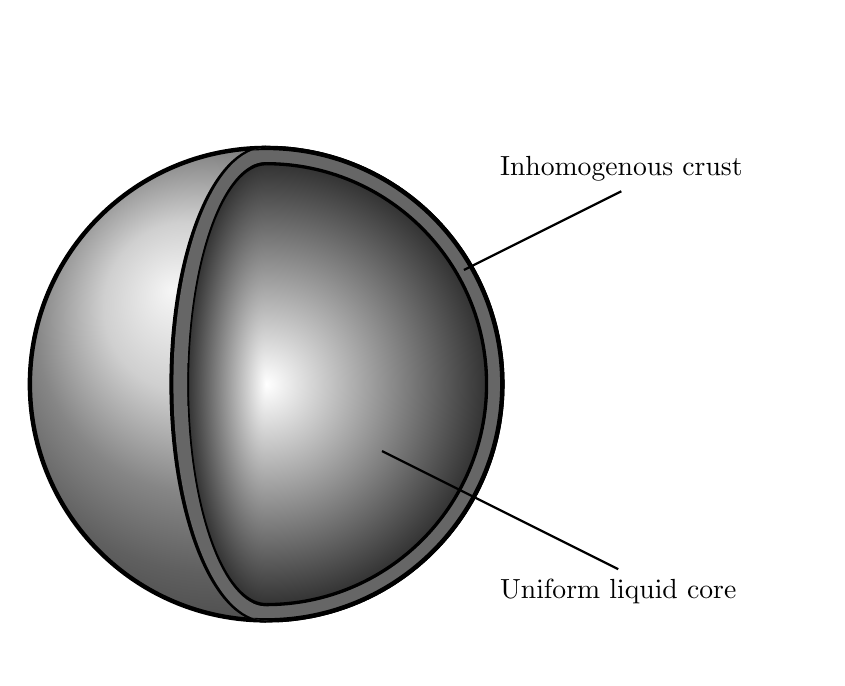
\begin{tikzpicture}[scale=1]
                \draw[ball color=gray!50,shading=ball, ultra thick, color=black] (0,0) circle (3cm);
                \draw[ultra thick] (0,3) arc (90:270:1.2cm and 3cm);
                \clip (0,-3) -- ++(7,-1) -- ++(0,8) -- ++(-7,-1) arc (90:270:1.177cm and 3cm) -- cycle;
                \draw[fill=gray!80!black, ultra thick] (0,0) circle (3cm); 
                \clip (0,-2.82) -- ++(7,-1) -- ++(0,7.64) -- ++(-7,-1) arc (90:270:1cm and 2.82cm) -- cycle;
                \shadedraw[draw=black, very thick,inner color=white, outer color=black!80] (0,0) circle (2.8cm);
                \draw[thick] (30:2.9cm) -- ++(2,1) node[above]{Inhomogenous crust};
                \draw[thick] (-30:1.7cm) -- ++(3,-1.5) node[below]{Uniform liquid core};
                \clip (0,2.82) arc (90:270:1.05cm and 2.82cm) -- cycle;
                \shadedraw[draw=black, very thick, inner color=white, outer color=black!80] (0,0) ellipse (1cm and 2.8cm);
        \end{tikzpicture}
        \caption{Neutron star's overall structure. The baryon density decreases (from white to dark gray) as we move outward from the \gls{NS} center.}
        \label{fig:NS_structure}
\end{figure} 

% \section{Tidal Deformation of Neutron Stars}%
% \label{sec:tidal_deformation_of_neutron_stars}

Following the gravitational wave (\gls{GW}) signals of the events GW170817 \citep{abbott2017gw170817} and GW190425 \citep{abbott2020gw190425} from two binary \gls{NS} mergers observed by LIGO and Virgo laser interferometer in 17\textsuperscript{th} August 2017 and 25\textsuperscript{th} April 2019 respectively, the tidal deformation of the \gls{NS} can be further constrained, as well as the mass $M$ and radius $R$ of the \gls{NS} \citep{abbott2018gw170817}. The \gls{NS} merger event is illustrated as in Figure \ref{fig:NS_merger}.

\begin{figure}[t]
        \centering
        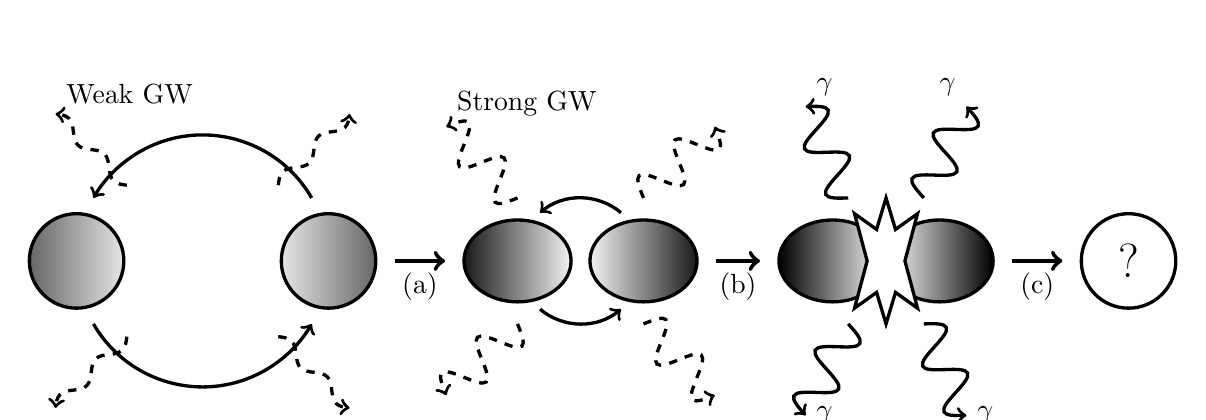
\begin{tikzpicture}[scale=0.8]
                \def\xl{-2};
                \def\xr{2};
                \def\r{0.75};
                \def\sep{3};
                \shadedraw[very thick, draw=black,left color=gray!80!black, right color=gray!20!white] (\xl,0) circle (\r cm);
                \shadedraw[very thick, draw=black,right color=gray!80!black, left color=gray!20!white] (\xr,0) circle (\r cm);
                \draw[->, very thick] (30:\xr cm) arc (30:150:\xr cm);
                \draw[->, very thick] (210:\xr cm) arc (210:330:\xr cm);
                \def\ang{-45};
                \draw[dashed, ->, very thick, cm={cos(\ang),-sin(\ang),sin(\ang),cos(\ang), (-\ang:1.7 cm)}] (0,0) sin (0.2,0.1) cos (0.4,0) sin (0.6,-0.1) cos (0.8,0) sin (1,0.1) cos (1.2,0) sin (1.4,-0.1) cos (1.6,0);
                \def\ang{-135};
                \draw[dashed, ->, very thick, cm={cos(\ang),-sin(\ang),sin(\ang),cos(\ang), (-\ang:1.7 cm)}] (0,0) sin (0.2,0.1) cos (0.4,0) sin (0.6,-0.1) cos (0.8,0) sin (1,0.1) cos (1.2,0) sin (1.4,-0.1) cos (1.6,0) node[above right]{Weak \gls{GW}};
                \def\ang{-225};
                \draw[dashed, ->, very thick, cm={cos(\ang),-sin(\ang),sin(\ang),cos(\ang), (-\ang:1.7 cm)}] (0,0) sin (0.2,0.1) cos (0.4,0) sin (0.6,-0.1) cos (0.8,0) sin (1,0.1) cos (1.2,0) sin (1.4,-0.1) cos (1.6,0);
                \def\ang{-315};
                \draw[dashed, ->, very thick, cm={cos(\ang),-sin(\ang),sin(\ang),cos(\ang), (-\ang:1.7 cm)}] (0,0) sin (0.2,0.1) cos (0.4,0) sin (0.6,-0.1) cos (0.8,0) sin (1,0.1) cos (1.2,0) sin (1.4,-0.1) cos (1.6,0);
                \draw[->, ultra thick] (\xr+\r+0.3,0) -- +(\sep-2*\r-0.7,0) node[pos=0.5,below]{(a)};

                \shadedraw[very thick, draw=black,left color=gray!20!black, right color=gray!10!white] (\xr+\sep,0) ellipse (0.85 cm and 0.65 cm);
                \shadedraw[very thick, draw=black,right color=gray!20!black, left color=gray!10!white] (\xr+\sep+2,0) ellipse (0.85 cm and 0.65 cm);
                \def\P{\xr+\sep+1};
                \def\R{1};
                \draw[->, very thick] (\P,0)+(50:\R cm) arc (50:130:\R cm);
                \draw[->, very thick] (\P,0)+(230:\R cm) arc (230:310:\R cm);
                \def\ang{-45};
                \draw[dashed, ->, very thick, cm={cos(\ang),-sin(\ang),sin(\ang),cos(\ang), (\P+1,1)}] (0,0) sin (0.2,0.3) cos (0.4,0) sin (0.6,-0.3) cos (0.8,0) sin (1,0.3) cos (1.2,0) sin (1.4,-0.3) cos (1.6,0);
                \def\ang{-135};
                \draw[dashed, ->, very thick, cm={cos(\ang),-sin(\ang),sin(\ang),cos(\ang), (\P-1,1)}] (0,0) sin (0.2,0.3) cos (0.4,0) sin (0.6,-0.3) cos (0.8,0) sin (1,0.3) cos (1.2,0) sin (1.4,-0.3) cos (1.6,0) node[above right]{Strong \gls{GW}};
                \def\ang{-225};
                \draw[dashed, ->, very thick, cm={cos(\ang),-sin(\ang),sin(\ang),cos(\ang), (\P-1,-1)}] (0,0) sin (0.2,0.3) cos (0.4,0) sin (0.6,-0.3) cos (0.8,0) sin (1,0.3) cos (1.2,0) sin (1.4,-0.3) cos (1.6,0);
                \def\ang{-315};
                \draw[dashed, ->, very thick, cm={cos(\ang),-sin(\ang),sin(\ang),cos(\ang), (\P+1,-1)}] (0,0) sin (0.2,0.3) cos (0.4,0) sin (0.6,-0.3) cos (0.8,0) sin (1,0.3) cos (1.2,0) sin (1.4,-0.3) cos (1.6,0);
                \draw[->, ultra thick] (\xr+\sep+2.85+0.3,0) -- +(\sep-2*0.85-0.6,0) node[pos=0.5,below]{(b)};

                \shadedraw[very thick, draw=black,left color=gray!0!black, right color=gray!0!white] (\xr+2*\sep+2,0) ellipse (0.85 cm and 0.65 cm);
                \shadedraw[very thick, draw=black,right color=gray!0!black, left color=gray!0!white] (\xr+2*\sep+3.7,0) ellipse (0.85 cm and 0.65 cm);
                \draw[->, ultra thick] (\xr+2*\sep+3.7+0.85+0.3,0) -- +(\sep-\r-0.85-0.6,0) node[pos=0.5,below]{(c)};
                \def\P{\xr+2*\sep+2.85};
                \draw[fill=white, very thick, shift={(\P,0)}] (0,1) -- (0.15,0.5) -- (0.5, 0.75) -- (0.3,0) -- (0.5,-0.75) -- (0.15,-0.5) -- (0,-1) -- (-0.15,-0.5) -- (-0.5,-0.75) -- (-0.3,0) -- (-0.5,0.75) -- (-0.15,0.5) -- cycle;
                \def\ang{-65};
                \draw[->, very thick, cm={cos(\ang),-sin(\ang),sin(\ang),cos(\ang), (\P+0.6,1)}] (0,0) sin (0.2,0.3) cos (0.4,0) sin (0.6,-0.3) cos (0.8,0) sin (1,0.3) cos (1.2,0) sin (1.4,-0.3) cos (1.6,0) node[above left]{$\gamma$};
                \def\ang{-115};
                \draw[->, very thick, cm={cos(\ang),-sin(\ang),sin(\ang),cos(\ang), (\P-0.6,1)}] (0,0) sin (0.2,0.3) cos (0.4,0) sin (0.6,-0.3) cos (0.8,0) sin (1,0.3) cos (1.2,0) sin (1.4,-0.3) cos (1.6,0) node[above right]{$\gamma$};
                \def\ang{-245};
                \draw[->, very thick, cm={cos(\ang),-sin(\ang),sin(\ang),cos(\ang), (\P-0.6,-1)}] (0,0) sin (0.2,0.3) cos (0.4,0) sin (0.6,-0.3) cos (0.8,0) sin (1,0.3) cos (1.2,0) sin (1.4,-0.3) cos (1.6,0) node[right]{$\gamma$};
                \def\ang{-295};
                \draw[->, very thick, cm={cos(\ang),-sin(\ang),sin(\ang),cos(\ang), (\P+0.6,-1)}] (0,0) sin (0.2,0.3) cos (0.4,0) sin (0.6,-0.3) cos (0.8,0) sin (1,0.3) cos (1.2,0) sin (1.4,-0.3) cos (1.6,0) node[right]{$\gamma$};

                \draw[very thick] (\xr+3.7+2*\sep+\sep,0) circle (\r cm) node{\LARGE ?};
        \end{tikzpicture}
        \caption{Illustration of binary \gls{NS} merger. (a) The two companion \glspl{NS} orbit about each others, while gradually losing energy through weak \gls{GW} and come closer with time. (b) As the two \gls{NS} get closer, they accelerate and emit stronger \gls{GW} until (c) colliding, which results in a \emph{kilonova}, characterized by a short \emph{gamma ray burst} (\gls{GRB}). The product of the merger has yet been decided to be a black hole (\gls{BH}) or another \gls{NS}.}
        \label{fig:NS_merger}
\end{figure} 
Apparently, the \gls{EoS} of high-density \gls{NM} plays the most important role in deciding the macroscopic properties of \gls{NS}. In particular, given the \gls{EoS} of the crust from the compressible liquid drop model and by using the \gls{EoS} of the uniform \gls{NS} core from the result of the \gls{HF} calculation of cold \textbeta-stable \gls{NM}, the gravitational mass and radius of the star can be decided by the framework of General Relativity (\gls{GR}) \citep{tan2020spin,tan2021equation}, i.e. the Tolman-Oppenheimer-Volkoff (\gls{TOV}) equation, which will in turn be compared to the observational astrophysical constraints to deduce the most suitable \gls{EoS} of the constituent \gls{NS} in this system.\par
In addition, due to the enormous mass, each \gls{NS} possesses powerful gravitational field and therefore, they tend to ``stretch out'' their companion under the tidal effect as in Figure \ref{fig:NS_merger}, while orbiting spirally toward each others and dissipating energy under the form of \gls{GW}. Particularly, the shape and mass-energy distribution of the \gls{NS} are tidally deformed from its supposedly spherical shape, resulting in nonzero multipole moments \citep{hinderer2008tidal,hinderer2010tidal,damour2009relativistic}. The \gls{NS}'s reaction, i.e. how strongly it deforms when being under a tidal field, is expressed in terms of the \emph{tidal Love numbers} $k_l$ of several orders $l$, where in this study, we will evaluate the Love number of \gls{NS} up to the 4\textsuperscript{th} order, i.e. $l=2,3,4$ \citep{perot2021role}. Apparently, the tidal Love number depends heavily on the \gls{EoS} of matter and this dependence will be further emphasized in Chapter \ref{chap:ns_prop}. For \gls{NS}, the central density can be up to $6n_0$ and possesses a Love number of order $\sim 0.1$, while our Earth has that of $0.3$. In a recent study, the Love number was calculated for spinning black holes, which showed that even with nearly infinite density, they still posess a small Love number of $0.002$ \citep{le2021spinning}.\par
Furthermore, under small perturbation of spacetime, the tidal field can also be separated into two components: the \emph{gravito-electric} (\gls{GE}) and \emph{gravito-magnetic} (\gls{GM}) terms \citep{damour2009relativistic} that are analogous to that in eletromagnetic field. As a result, the deformation of the \gls{NS}, i.e. Love numbers, in the perturbed tidal field can also be categorized into the corresponding \gls{GE} ($k_l$) and \gls{GM} ($j_l$) components \citep{perot2021role}, whose result will be presented in more details in Chapter \ref{chap:ns_prop}. To sum up, this study is dedicated to:
\begin{itemize}
        \item Include the spin polarization effect to the existing CDM3Y$n$ and BDM3Y1 models \citep{tan2021equation},
        \item Assess the dependence of \gls{NS}'s gravitational mass and radius to different \gls{EoS},
        \item Investigate the sensitivity of \gls{GE} and \gls{GM} tidal deformability and Love numbers to \gls{NM} properties,
        \item Compare some of the \gls{NS}'s calculated properties to the empirical astrophysical constraints obtained in recent studies \citep{abbott2018gw170817,xie2019bayesian}.
\end{itemize}


        \chapter{Hartree-Fock Formalism of Nuclear Matter}
        \label{chap:hf}
        \section{Nucleon-Nucleon Interaction}%
\label{sec:nucleon_nucleon_interaction}

Due to the lack of a exact theory to describe the nucleon-nucleon (\gls{NN}) interaction, a model need to be imposed and fit with experimental measurement or theoretical calculation results. Plus, for a system as massive as a \gls{NS}, deducing the \gls{EoS} using the \emph{ab initio} method, i.e. solving the Schr\"{o}dinger equation over all particles, is simply impossible, therefore an \emph{effective interaction} must be used \citep{greiner1996nuclear}. In this section, we only limit ourselves to two-body interaction, thus, the \gls{NN} potential can be expressed in the form of
\begin{equation}
        v = v(\bm{r}, \bm{r'}, \bm{p}, \bm{p'}, \bm{\sigma}, \bm{\sigma'}, \bm{\tau}, \bm{\tau'})
        \label{eff_interaction}
\end{equation}
where the primed and unprimed variables indicate the properties of 2 nucleons respectively, in which $\bm{r}$ is the particle's position, $\bm{p}$ is its momentum, $\bm{\sigma}$ is its intrinsic spin and $\bm{\tau}$ is its isospin.\par
The functional form of $v$ in \eqref{eff_interaction} cannot freely take any form but is constrained by many invariance requirements \citep{greiner1996nuclear}
\begin{itemize}
        \item \textbf{Translational invariance:} The \gls{NN} potential should only depend on the \emph{relative position} of the two particle but not their explicit positions, thus we can reduce \eqref{eff_interaction} to
                \begin{equation}
                        v = v(\bm{r}-\bm{r'},\bm{p},\bm{p'},\bm{\sigma},\bm{\sigma'},\bm{\tau},\bm{\tau'}) = v(\bm{r},\bm{p},\bm{p'},\bm{\sigma},\bm{\sigma'},\bm{\tau},\bm{\tau'})
                \end{equation}
                with at the last expression, we redefine $\bm{r}$ as the relative position vector.

        \item \textbf{Galilei invariance:} The potential should also be invariant under transformation between inertial frame of reference, which requires that only the relative momentum $\bm{p}-\bm{p'}$ is depended, i.e.
                \begin{equation}
                        v = v(\bm{r},\bm{p},\bm{\sigma},\bm{\sigma'},\bm{\tau},\bm{\tau'})
                        \label{eq2-3}
                \end{equation}
                where here we denote $\bm{p}$ as the relative momentum.

        \item \textbf{Rotational invariance:} The potential should be constructed such that the total angular momentum is zero.
                
        \item \textbf{Isospin invariance:} The \gls{NN} interaction potential needs to be invariant under rotation in isospin space, in other words, it can only depend on the isospin-independent terms and the terms with $\bm{\tau}\cdot\bm{\tau'}$. Therefore, we can split the potential into
                \begin{equation}
                        v = v_0 (\bm{r},\bm{p},\bm{\sigma},\bm{\sigma'}) + v_1 (\bm{r},\bm{p},\bm{\sigma},\bm{\sigma'}) \bm{\hat{\tau}}\cdot\bm{\hat{\tau}'}
                \end{equation}

        \item \textbf{Parity invariance:} The \gls{NN} interaction potential is also expected to be invariant under the action of parity operator, i.e. changing the sign of spatial coordinates
                \begin{equation}
                        v(\bm{r},\bm{p},\bm{\sigma},\bm{\sigma'},\bm{\tau},\bm{\tau'}) = v(-\bm{r},-\bm{p},\bm{\sigma},\bm{\sigma'},\bm{\tau},\bm{\tau'})
                \end{equation}

        \item \textbf{Time reversal invariance:} Finally, the interaction should stay the same after switching the time arrow direction
                \begin{equation}
                        v(\bm{r},\bm{p},\bm{\sigma},\bm{\sigma'},\bm{\tau},\bm{\tau'}) = v(\bm{r},-\bm{p},-\bm{\sigma},-\bm{\sigma'},\bm{\tau},\bm{\tau'})
                \end{equation}
\end{itemize}
Having the above considerations, developing further the M3Y-Paris interaction, which was used by the \gls{HF} study of \gls{NM} \citep{loan2011equation, tan2016mean, tan2020spin,tan2021equation} and the folding model study of \gls{NN} scattering \citep{khoa1997nuclear,khoa2000generalized},
\begin{equation}
        v = v_{00}(r) + v_{10}(r) \bm{\sigma}\cdot\bm{\sigma'} + v_{01}(r) \bm{\tau}\cdot\bm{\tau'} + v_{11}(r) (\bm{\sigma}\cdot\bm{\sigma'})(\bm{\tau}\cdot\bm{\tau'})
\end{equation}
by adding a density-dependent form factor to each term gives the CDM3Y$n$ interaction model
\begin{IEEEeqnarray*}{rCl}
        v(\rho,r) &=& F_{00}(\rho) v_{00}(r) + F_{10}(\rho) v_{10}(r) \bm{\sigma}\cdot\bm{\sigma'}\\
          &&\negmedspace{}+ F_{01}(\rho) v_{01}(r) \bm{\tau}\cdot\bm{\tau'} + F_{11}(\rho) v_{11}(r) (\bm{\sigma}\cdot\bm{\sigma'})(\bm{\tau}\cdot\bm{\tau'})\IEEEyesnumber
          \label{eq2-11}
\end{IEEEeqnarray*}  
where each radial term is the superposition of 3 Yukawa potentials
\begin{equation}
        v_{\sigma\tau}(r) = \sum^{3}_{k=1} Y_{\sigma\tau}(k) \frac{\exp(-\mu_k r)}{\mu_k r} 
\end{equation}
and the form factor $F_{\sigma\tau}(\rho)$ shared the functional form \citep{khoa1997nuclear,tan2020spin,tan2021equation,than2010ufr}
\begin{equation}
        F_{\sigma\tau}(\rho) = C_{\sigma\tau} [1 + \alpha_{\sigma\tau} \exp(-\beta_{\sigma\tau}\rho) + \gamma_{\sigma\tau}\rho]
\end{equation}
with parameters given in Table \ref{tab:cd}. The parameters of $F_{00}$ were adjusted to give the corresponding incompressibility $K$ of symmetric \gls{NM} at saturation density $\rho_0$ and the binding energy $E_0 \approx 15.8\; MeV$, while the 10 term is modified from \citep{than2010ufr} to reproduce $E_{sym}(\rho_0) \approx 30\;MeV$, $L\approx 50\;MeV$ and to be in agreement with the ab-initio results \citep{akmal1998equation,gandolfi2010microscopic} at higher density \citep{tan2021equation}. On the other hand, the spin-dependent terms, 10 and 11, are hereby included in the 5 models by fine tuning the parameters to yield the same result as the Brueckner-Hartree-Fock (\gls{BHF}) study of spin polarized \gls{NM} \citep{vidana2002equation} as in Figure \ref{fig:bhf}.

\begin{figure}[t]
        \centering
        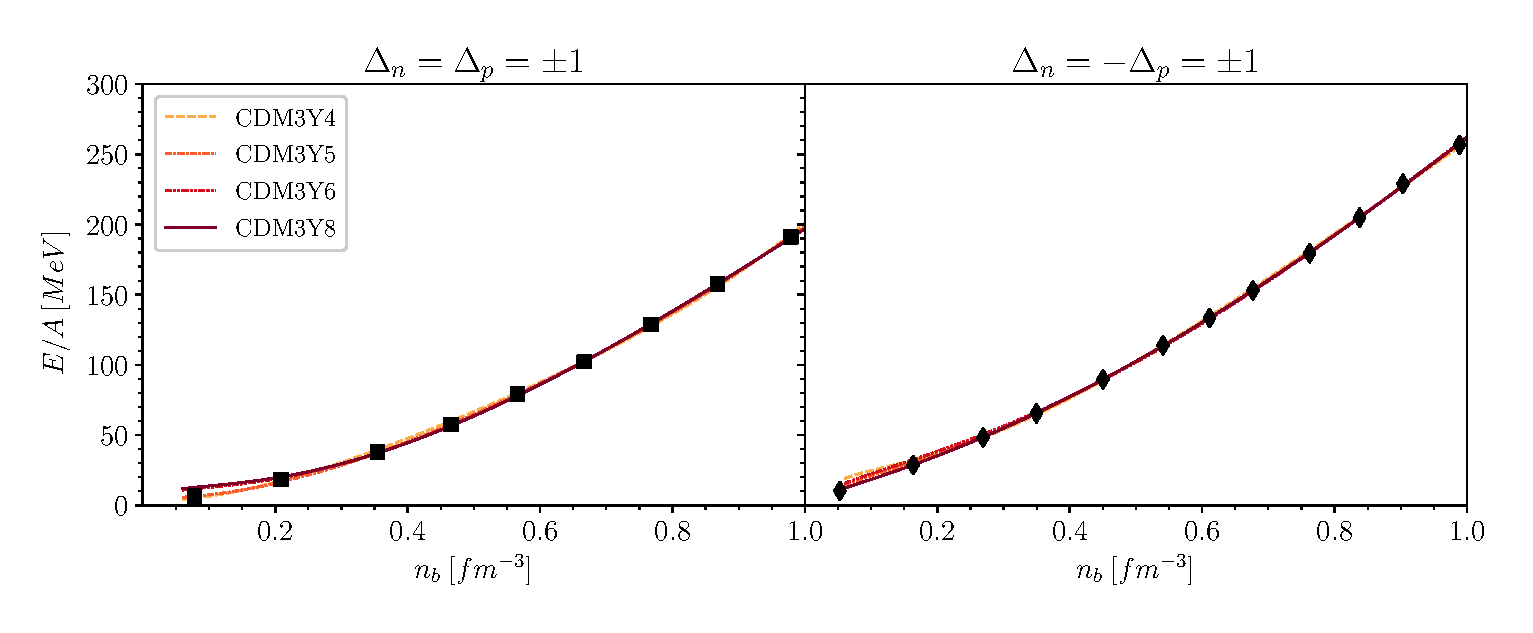
\includegraphics[width=\textwidth]{fig/BHF_fit.eps}
        \caption{Energy per baryon $E/A$ of symmetric \gls{NM} by the 5 CDM3Y$n$ models compared to \gls{BHF} result \citep{vidana2002equation}. The diamond and square represent the \gls{BHF} result for $\Delta_n=-\Delta_p=\pm 1$ and $\Delta_n=\Delta_p=\pm 1$ respectively with $\Delta_\tau$ being the baryon spin polarity.}
        \label{fig:bhf}
\end{figure} 

\begin{table}[H]
        \centering
        \caption{CDM3Y$n$ interaction's parameters; the 00 and 01 terms are inherited from \citep{tan2021equation}, while the 10 and 11 parameters are added by fitting with \gls{BHF} result.}
        \label{tab:cd}
        \begin{tabular}{|C|C|C|C|C|C|C|}
                \hline
                \text{Interaction} & \sigma\tau & C_{\sigma\tau} & \alpha_{\sigma\tau} & \beta_{\sigma\tau} & \gamma_{\sigma\tau} & K\\
                                   & & & & (fm^3) & (fm^3) & (MeV)\\
                \hline
                \multirow{4}{*}{\text{CDM3Y3}} & 00 & 0.2985 & 3.4528 & 2.6388 & -1.5 &\multirow{4}{*}{217}\\
                                               & 01 & 0.2343 & 5.3336 & 6.4738 & 4.3172 &\\
                                               & 10 & 0.3890 & 3.5635 & -2.6717 & 20.3624 &\\
                                               & 11 & 0.8802 & 4.0433 & 12.3262 & 0.3662 &\\
                \hline
                \multirow{4}{*}{\text{CDM3Y4}} & 00 & 0.3052 & 3.2998 & 2.3180 & -2.0 &\multirow{4}{*}{228}\\
                                               & 01 & 0.2129 & 6.3581 & 7.0584 & 5.6091 &\\
                                               & 10 & 0.2593 & 6.0016 & -2.3377 & 18.8725 &\\
                                               & 11 & 0.8329 & 3.5941 & 9.2012 & 0.2690 &\\
                \hline
                \multirow{4}{*}{\text{CDM3Y5}} & 00 & 0.2728 & 3.7367 & 1.8294 & -3.0 &\multirow{4}{*}{241}\\
                                               & 01 & 0.2204 & 6.6146 & 7.9910 & 6.0040 &\\
                                               & 10 & 0.4106 & 5.6265 & -1.6698 & -1.9866 &\\
                                               & 11 & 0.6815 & 2.5833 & 5.1700 & 0.2578 &\\
                \hline
                \multirow{4}{*}{\text{CDM3Y6}} & 00 & 0.2658 & 3.8033 & 1.4099 & -4.0 &\multirow{4}{*}{252}\\
                                               & 01 & 0.2313 & 6.6865 & 8.6775 & 6.0182 &\\
                                               & 10 & 0.5186 & 9.9402 & 1.6698 & 2.9799 &\\
                                               & 11 & 0.6058 & 3.1947 & 4.4512 & 0.0822 &\\
                \hline
                \multirow{4}{*}{\text{CDM3Y8}} & 00 & 0.2658 & 3.8033 & 1.4099 & -4.3 &\multirow{4}{*}{257}\\
                                               & 01 & 0.2643 & 6.3836 & 9.8950 & 5.4249 &\\
                                               & 10 & 0.5997 & 9.1900 & 0.7514 & -4.7181 &\\
                                               & 11 & 0.3786 & 3.9435 & 2.7012 & 0.3512 &\\
                \hline
        \end{tabular}
\end{table}

\section{Equation of States of Nuclear Matter}%
\label{sec:equation_of_states_of_nuclear_matter}

In \gls{HF} formalism, the total \gls{HF} energy of the system can be expressed as
\begin{IEEEeqnarray*}{rCl}
        E_{HF} &=& \sum^{}_{\sigma\tau} \sum^{k_F^{\sigma\tau}}_{\bm{k}} \frac{\hbar^2 k^2}{2m_\tau} + \frac{1}{2} \sum^{}_{\bm{k}\sigma\tau} \sum^{}_{\bm{k'}\sigma'\tau'} \left[ \mel**{\bm{k}\sigma\tau,\bm{k'}\sigma'\tau'}{v^D}{\bm{k}\sigma\tau,\bm{k'}\sigma'\tau'} \right.\\
          && \left. \negmedspace{} + \mel**{\bm{k}\sigma\tau,\bm{k'}\sigma'\tau'}{v^{EX}}{\bm{k'}\sigma\tau,\bm{k}\sigma'\tau'} \right]\IEEEyesnumber
          \label{eqE}
\end{IEEEeqnarray*}  
where the single-particle wave function is plane wave
\begin{equation}
        \ket{\bm{k}\sigma\tau} = \frac{e^{i\bm{k}\cdot\bm{r}}}{ \sqrt{ \Omega}  } \chi_\sigma \chi_\tau
\end{equation}
$\Omega$ being the spatial volume of the system, $k_F^{\sigma\tau} = (6\pi^2 \rho_{\sigma\tau})^{1/3}$ is the Fermi momentum corresponding to spin $\sigma$ and isospin $\tau$, $v^{D(EX)}$ is the direct (exchange) part of the interaction determined from the singlet and triplet-even (odd) of the central \gls{NN} force. Adopting the same functional form of \eqref{eq2-11}, the direct and exchange interaction is written as
\begin{IEEEeqnarray*}{rCl}
        v^{D(EX)}(\rho_b,r) &=& F_{00}(\rho_b) v^{D(EX)}_{00}(r) + F_{10}(\rho_b) v^{D(EX)}_{10}(r) \bm{\sigma}\cdot\bm{\sigma'}\\
                          &&\negmedspace{}+ F_{01}(\rho_b) v^{D(EX)}_{01}(r) \bm{\tau}\cdot\bm{\tau'} + F_{11}(\rho_b) v^{D(EX)}_{11}(r) (\bm{\sigma}\cdot\bm{\sigma'})(\bm{\tau}\cdot\bm{\tau'})\IEEEyesnumber
                          \label{eqHF}
\end{IEEEeqnarray*}
and
\begin{IEEEeqnarray*}{rCl}
        v^{D(EX)}_{\sigma\tau}(r) &=& \sum^{3}_{k=1} Y^{D(EX)}_{\sigma\tau}(k) \frac{\exp(-\mu_k r)}{\mu_k r} \IEEEyesnumber
\end{IEEEeqnarray*}  
with the Yukawa strengths given in Table \ref{tab:yukawa} and the density-dependent form factor parameters are in Table \ref{tab:cd}. Note that in \eqref{eqHF}, $\rho_b$ denotes the \emph{baryon density}, this will be used in order to distinguish with the lepton density in the later section.

\begin{table}[H]
        \centering
        \caption{Yukawa strengths of the M3Y-Paris interaction \citep{tan2020spin,anantaraman1983effective}.}
        \label{tab:yukawa}
        \begin{tabular}{|C|C|C|C|C|C|C|C|C|C|}
                \hline
                k & \mu_k & Y^D_{00} & Y^D_{10} & Y^D_{01} & Y^D_{11} & Y^{EX}_{00} & Y^{EX}_{10} & Y^{EX}_{01} & Y^{EX}_{11}\\
                    & (fm^{-1}) & (MeV) & (MeV) & (MeV) & (MeV) & (MeV) & (MeV) & (MeV) & (MeV)\\
                \hline
                1 & 4.0& 11061.625 & 938.875 & 313.625 & -969.125 & -1524.25 & -3492.75 & -4118.0 & -2210.0\\
                2 & 2.5 & -2537.5 & -36.0 & 223.5 & 450.0 & -518.75 & 795.25 & 1054.75 & 568.75\\
                3 & 0.7072 & 0.0 & 0.0 & 0.0 & 3.4877 & -7.8474 & 2.6157 & 2.6157 & -0.8719\\
                \hline
        \end{tabular}
\end{table}
Multiply \eqref{eqE} with $\Omega^{-1}$, the energy density of the \gls{NM} is separated into the kinetic term $\varepsilon_{kin}$ and the potential terms $\varepsilon_{\sigma\tau}$, i.e.
\begin{equation}
        \varepsilon_{HF} = \frac{E_{HF}}{\Omega} = \varepsilon_{kin} + F_{00}(\rho_b) \varepsilon_{00} + F_{01}(\rho_b) \varepsilon_{01} + F_{10}(\rho_b) \varepsilon_{10} + F_{11}(\rho_b) \varepsilon_{11}
\end{equation}
The final expressions of each terms of the energy density are
\begin{IEEEeqnarray}{rCl}
        \varepsilon_{kin} &=& \frac{3}{10} \sum^{}_{\sigma\tau} \frac{\hbar^2 (k_F^{\sigma\tau})^2}{m_\tau} \rho_{\sigma\tau}\\
        \varepsilon_{00} &=& \frac{1}{2} \left[ \rho_b^2 J^D_{00} + \int {A^2_{00} v^{EX}_{00}(r)} \: d^3 r \right] \\
        \varepsilon_{10} &=& \frac{1}{2} \left[ \rho_b^2 J^D_{10} \left( \Delta_n \frac{1+\delta}{2} + \Delta_p \frac{1-\delta}{2} \right)^2 + \int {A^2_{10} v^{EX}_{10}(r)} \: d^3 r \right] \\
        \varepsilon_{01} &=& \frac{1}{2} \left[ \rho_b^2 J^D_{01}\delta^2 + \int {A^2_{01} v^{EX}_{01}(r)} \: d^3 r \right] \\
        \varepsilon_{11} &=& \frac{1}{2} \left[ \rho_b^2 J^D_{11} \left( \Delta_n \frac{1+\delta}{2} - \Delta_p \frac{1-\delta}{2} \right)^2 + \int {A^2_{11} v^{EX}_{11}(r)} \: d^3 r \right]
\end{IEEEeqnarray}  
where $\Delta_{\tau} = (\rho_{\uparrow \tau} - \rho_{\downarrow \tau})/\rho_{\tau}$ is the polarity of nucleon, $\delta = (\rho_n - \rho_p)/\rho_b$ is the asymmetry of \gls{NM}, $J^D_{\sigma\tau} = \int v^D_{\sigma\tau}(r)\: d^3 r$ is the volume integral of the direct interaction and
\begin{equation}
        \begin{array}{l}
                A_{00} = \rho_{\uparrow n} \hat{j_1}(k_F^{\uparrow n} r) + \rho_{\downarrow n} \hat{j_1}(k_F^{\downarrow n} r) + \rho_{\uparrow p} \hat{j_1}(k_F^{\uparrow p} r) + \rho_{\downarrow p} \hat{j_1}(k_F^{\downarrow p} r)\\[5pt]
                A_{10} = \rho_{\uparrow n} \hat{j_1}(k_F^{\uparrow n} r) - \rho_{\downarrow n} \hat{j_1}(k_F^{\downarrow n} r) + \rho_{\uparrow p} \hat{j_1}(k_F^{\uparrow p} r) - \rho_{\downarrow p} \hat{j_1}(k_F^{\downarrow p} r)\\[5pt]
                A_{01} = \rho_{\uparrow n} \hat{j_1}(k_F^{\uparrow n} r) + \rho_{\downarrow n} \hat{j_1}(k_F^{\downarrow n} r) - \rho_{\uparrow p} \hat{j_1}(k_F^{\uparrow p} r) - \rho_{\downarrow p} \hat{j_1}(k_F^{\downarrow p} r)\\[5pt]
                A_{11} = \rho_{\uparrow n} \hat{j_1}(k_F^{\uparrow n} r) - \rho_{\downarrow n} \hat{j_1}(k_F^{\downarrow n} r) - \rho_{\uparrow p} \hat{j_1}(k_F^{\uparrow p} r) + \rho_{\downarrow p} \hat{j_1}(k_F^{\downarrow p} r)
        \end{array}
\end{equation}
with $\hat{j}_1(x)=3j_1(x)/x$ and $j_1(x)$ being the 1\textsuperscript{st} order spherical Bessel function.

\section{\textbeta-Stable Nuclear Matter}%
\label{sec:textbeta_stable_nuclear_matter}

After the \gls{HF} calculation, we were able to obtain a numerical \gls{HF} energy density $\varepsilon(\rho_n,\rho_p,\Delta_n,\Delta_p)$. However, it is in fact impossible for a \gls{NS} to exist while consisting of purely nucleon. In order to compensate for this issue, leptons ($e^-$ and $\mu^-$) have to be introduced to the matter constituents and the $npe\mu$ matter has to satisfy the \emph{\textbeta-stable} condition \citep{glendenning2012compact}, i.e.
\begin{itemize}
        \item Charge balance
                \begin{equation}
                        \rho_p = \rho_e + \rho_\mu
                        \label{chargeEQ}
                \end{equation}
        \item Chemical potential balance
                \begin{equation}
                        \mu_n - \mu_p = \mu_e = \mu_\mu
                \end{equation}
                where $\mu_i = \pdv{\varepsilon}{\rho_i}$ ($i=n,p,e,\mu$) is the chemical potential of the $i$ particle.
\end{itemize}
The total energy density of the $npe\mu$ matter is thus
\begin{equation}
        \varepsilon = \varepsilon_{HF} + \rho_n m_n c^2 + \rho_p m_p c^2 + \varepsilon_e + \varepsilon_\mu 
\end{equation}
which leads to the nucleon chemical potential of the form
\begin{equation}
        \mu_\tau (\rho_n,\rho_p,\Delta_n,\Delta_p) = \frac{\partial \varepsilon}{\partial \rho_\tau}  = \frac{\partial \varepsilon_{HF}}{\partial \rho_\tau} + m_\tau c^2
\end{equation}
Let $\hat{\mu} = \mu_n - \mu_p$ be the leptons' chemical potential, \eqref{chargeEQ} is equivalent to\footnote{$\theta(x)$ is the Heaviside function, i.e. it returns $1$ for $x\geq 0$ and $0$ otherwise.}
\begin{equation}
        3\pi^2 (\hbar c)^3 \rho_p - \hat{\mu}^3 - \left[ \hat{\mu}^2 - (m_\mu c^2)^2 \right]^{3/2} \theta(\hat{\mu} - m_\mu c^2) = 0
\end{equation}
from which the proton fraction $x_p = \rho_p/\rho_b$ can be obtained as shown in Figure \ref{fig:xp}. Furthermore, under strong magnetic field like that of a magnetar, we can approximate $\Delta_n \approx -\Delta_p \approx \Delta$ and reduce the \gls{EoS} to depend on just the baryon polarity $\Delta$ alone, and the more baryon polarized, the stronger the magnetic field of the \gls{NS}.\par
For a fixed value of $\Delta$, we are able to obtain a density function of the form $\rho_n (\rho_b, \Delta)$ and $\rho_p (\rho_b, \Delta)$, which in turn gives the lepton chemical potential $\hat{\mu}(\rho_b,\Delta) = \hat{\mu}(\rho_n,\rho_p)$ On the other hand, the leptons' densities are then \cite{loan2011equation}
\begin{equation}
        \rho_e(\rho_b,\Delta) = \frac{ \hat{\mu}^3(\rho_b,\Delta)}{ 3\pi^2 (\hbar c)^3} \quad\text{and}\quad \rho_\mu(\rho_b,\Delta) = \frac{ \Big[\hat{\mu}^2(\rho_b,\Delta) - (m_\mu c^2)^2\Big]^{3/2}}{ 3\pi^2 (\hbar c)^3} \theta(\hat{\mu}(\rho_b,\Delta)-m_\mu c^2)
\end{equation} 
Consider the $e^-$ and $\mu^-$ to be systems of relativistic Fermi gas, then their respective energy densities and pressure contributions are ($l=e,\mu$) \citep{moustakidis2009equation}
\begin{equation}
        \varepsilon_l(\rho_b,\Delta) = \frac{ 2}{ (2\pi)^3} \int_{{0}}^{{[3\pi^2\rho_l(\rho_b,\Delta)]^{1/3}}} {\sqrt{\hbar^2 c^2 k^2 + m_l^2 c^4}} \: d^3{\mathbf{k}}
\end{equation} 
and
\begin{equation}
        P_l(\rho_b,\Delta) = \frac{ 1}{ 3} \frac{ 2}{ (2\pi)^3} \int_{{0}}^{{[3\pi^2 \rho_l(\rho_b,\Delta)]^{1/3}}} { \frac{ \hbar^2 c^2 k^2}{ \sqrt{\hbar^2 c^2 k^2 + m_l^2 c^4}} } \: d^3{\mathbf{k}}
\end{equation} 
Plus, from the \gls{HF} formalism with \gls{NM}, the baryon pressure is given by
\begin{equation}
        P_b = \rho_b^2 \pdv{(\varepsilon_{HF}/\rho_b)}{\rho_b}
\end{equation}
Finally, we obtain the total energy density dependence on baryon density as 
\begin{equation}
        \varepsilon(\rho_b,\Delta) = \varepsilon_{HF}(\rho_b,\Delta) + \rho_n(\rho_b,\Delta)m_n c^2 + \rho_p(\rho_b,\Delta)m_p c^2 + \varepsilon_e(\rho_b,\Delta) + \varepsilon_\mu(\rho_b,\Delta)
\end{equation}
and the total pressure of \gls{NS} matter
\begin{equation}
        P(\rho_b,\Delta) = P_b(\rho_b,\Delta) + P_e(\rho_b,\Delta) + P_\mu(\rho_b,\Delta)
\end{equation}
and this completes the \gls{EoS} of cold $\beta$-stable \gls{NS} matter (Figure \ref{fig:e} and \ref{fig:p}).


        \chapter{Neutron Star Properties}
        \label{chap:ns_prop}
        The observation of the NS merger GW170817 has provided for the first time the empirical
estimate of the tidal deformation of NS induced by strong gravitational field between 
the two companions of a merging binary pulsar \citep{hinderer2008tidal,hinderer2010tidal}. 
In this chapter, 
we discuss briefly, within the frame of General Relativity, how a static spherical NS can be
tidally deformed by gravitation, gaining nonzero gravito-multipole moments which are
directly proportional to the strength of gravitation \citep{damour2009relativistic}.
The tidal deformation moments of different multipoles are determined in the present work 
with the mean-field based EoS of spin-polarized NS matter using the explicit expressions 
of the Love numbers given by GR \citep{perot2021role}. The obtained results for the tidal
deformability as well as the gravitational mass $M$ and radius $R$ of \gls{NS} are 
compared in details with the astrophysical constraints deduced from the observation 
of GW170817.

\section{Einstein equations of relativistic neutron star}%
\label{sec3.1}
In general, the line element of metric in the static isotropic spacetime can be 
expressed within GR  \citep{oppenheimer1939massive} in terms of spatial spherical 
coordinates as
\begin{equation}
        ds^2 = g_{\mu\nu}dx^\mu dx^\nu= - e^{2\nu(r)}c^2dt^2 + e^{2\lambda(r)}dr^2 + 
				r^2 d\theta^2 + r^2\sin^2\theta d\phi^2, \label{metr}
\end{equation}
where arbitrary functions $\nu(r)$ and $\lambda(r)$ are determined locally by the
mass-energy density enclosed within the sphere of radius $r$. In the vicinity of a 
static spherical NS, the spacetime geometry is determined from the pressure and 
mass-energy density of NS matter (treated as a perfect fluid), and the  
energy-momentum tensor is obtained in \gls{GR} as
\begin{equation}
        T^{\mu\nu}= Pg^{\mu\nu} + (P+\rho) u^\mu u^\nu,\quad
				g_{\mu\nu}u^\mu u^\nu=u_\nu u_\nu=-1.
\end{equation}
Here $P$ and $\rho$ are the pressure and mass-energy density of NS matter, respectively,
$u^\mu = dx^\mu/d\tau$ is the local fluid 4-velocity. The Einstein's field 
equations of neutron star are written as 
\begin{equation}
        G^{\mu\nu} = \frac{8\pi G}{c^4} T^{\mu\nu}. \label{Ein} 
\end{equation}
Keeping the nonrelativistic limit to the static Newtonian gravitation, the 
Einstein's field equations (\ref{Ein}) can be reduced to the following differential 
equations which are known as Tolman-Oppenheimer-Volkoff (\gls{TOV}) equations 
\citep{oppenheimer1939massive}
\begin{eqnarray}
\frac{d P(r)}{dr}&=& -\frac{G \rho(r)\mathcal{M}(r)}{c^2 r^2} 
 \left[ 1+\frac{P(r)}{\rho(r)}\right] 
\left[1+\frac{4 \pi P(r) r^3}{c^2 \mathcal{M}(r)} \right] 
\left[ 1-\frac{2G \mathcal{M}(r)}{c^2 r} \right]^{-1}, \nonumber \\
d\mathcal{M}(r) &=& 4\pi r^2 \rho(r)dr, \label{tov} 
\end{eqnarray}
where $r$ is the radial coordinate in Schwarzschild metric (\ref{metr}), and 
$\mathcal{M}(r)$ is the gravitational mass enclosed within sphere of radius $r$. 
$\rho(r)$ and $P(r)$ are the mass-energy density and pressure of NS matter at 
distance $r$ from the star center, respectively. The \gls{TOV} equations (\ref{tov}) are 
integrated from $r=0$ to the surface of NS, with the star radius $R$ given by 
$P(R)=0$. Other boundary conditions are 
\begin{align}
\mathcal{M}(0)=0, \quad \rho(0)=\rho_{\rm c}, \quad P(0)=P_{\rm c},\quad \mathcal{M}(R)=M.   
\label{Bdr}
\end{align}
From the solutions of the \gls{TOV} equations \eqref{tov} based on the pressure and mass-energy
density of \gls{NS} matter given by the considered \gls{EoS}, the correlated profiles of the mass 
and pressure of \gls{NS} can be obtained as functions of distance $r$ from the star center. 
The total mass $M$ and radius $R$ of \gls{NS} are then deduced from the boundary conditions 
for the \gls{TOV} solutions.

\subsection*{Partial spin polarization of baryons in NS matter}
The \gls{HF} results in Chap \ref{chap:hf} have been obtained with the uniform (density independent)  
spin polarization of baryons of different strengths $\Delta$. However, the magnetic 
field distribution inside a magnetar is much more complex \citep{fujisawa2014magnetic}, 
and the use of a density independent $\Delta$ cannot be justified. In fact, baryons in the 
inner core of the magnetar are tightly compressed by gravity at high densities of \gls{NS} matter
which leads to the full degeneracy so that there is no possibility for baryon to flip 
its spin orientation. Therefore, along with the intrinsic magnetic field, the spin 
polarization of baryons is expected to gradually weaken to $\Delta \approx 0$ at high
densities in the center of \gls{NS} \citep{fujisawa2014magnetic,tan2020spin}. Although it's beyond 
the scope of the current study to precisely calculate the density dependence of $\Delta(n_b)$, 
we explore this effect by investigating two different scenarios proposed recently by
\cite{tan2020spin}, based on the magnetic field distribution of magnetar modelled by 
\cite{fujisawa2014magnetic}
\begin{enumerate}[label=(\Alph*)]
    \item The magnetic field is strongly localized in the surface region of the magnetar, 
		near the crust-core transition, and $\Delta\to 0$ at $n_b\approx 0.18$ fm$^{-3}$,
    \item The magnetic field distribution is broader, covering both the crust and outer 
        core of \gls{NS}, and $\Delta$ decreases gradually to zero at a larger density 
		$n_b \approx 0.35$ fm$^{-3}$. 
\end{enumerate}
\begin{figure}[ht!]
    \centering
    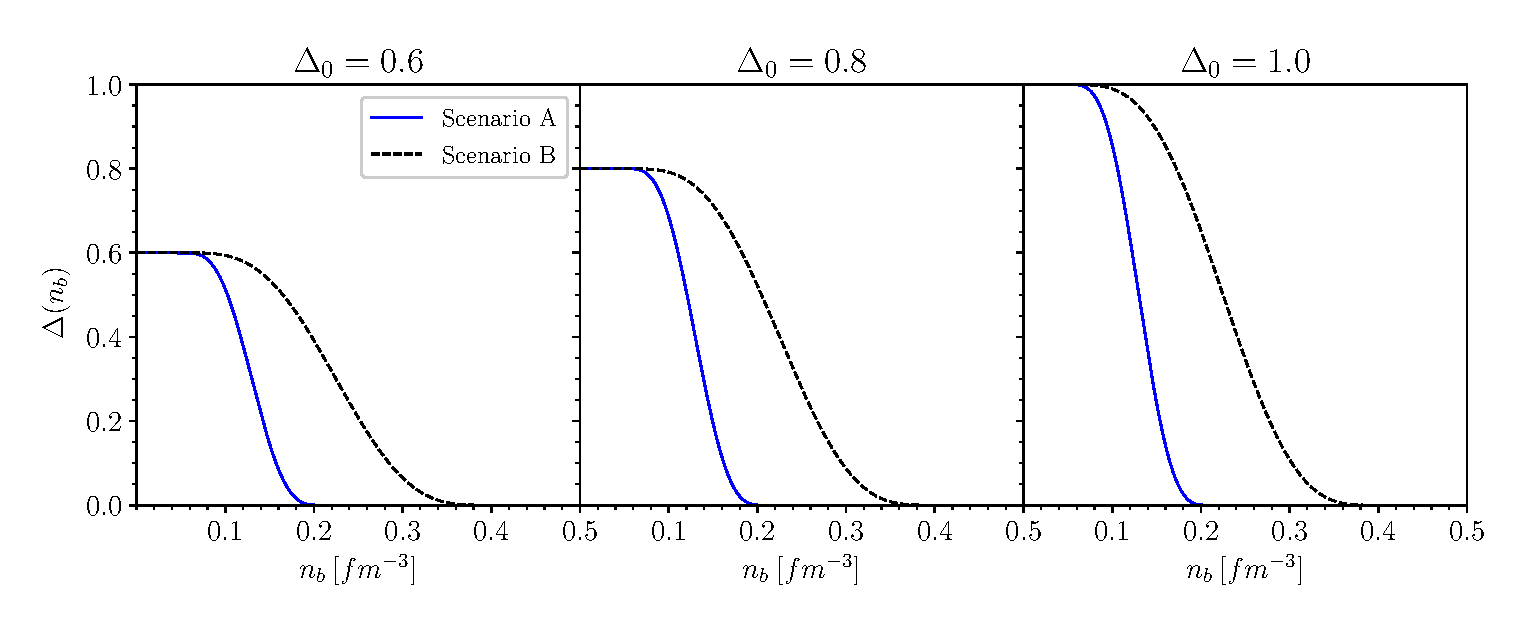
\includegraphics[width=\textwidth]{fig/Delta.eps}
    \caption{Different scenarios of the density dependence of the spin polarization 
		of baryons.}
    \label{fig:Delta}
\end{figure} 
\begin{figure}[ht!]
        \centering
        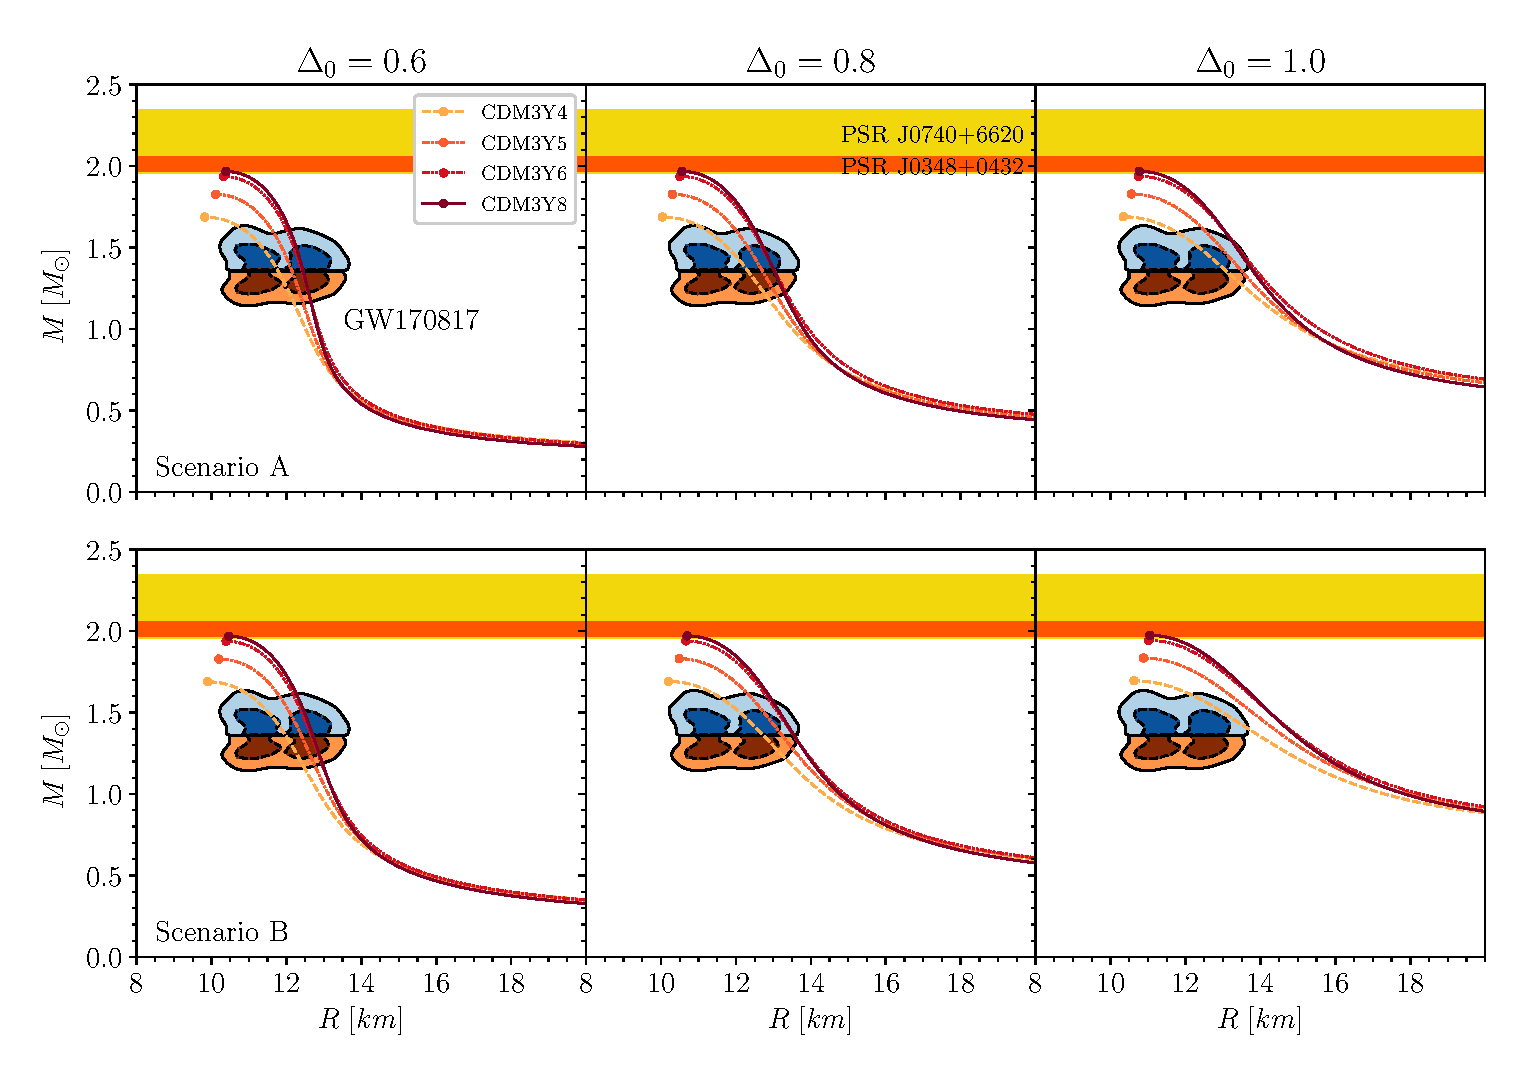
\includegraphics[width=\textwidth]{fig/MR.eps}
        \caption{The correlation of the gravitational mass $M$ and radius $R$ of magnetar 
            given by the solutions of the \gls{TOV} equations (\ref{tov}) obtained with different 
            EoS's of spin-polarized \gls{NS} matter. The empirical constraints for \gls{NS} with 
				mass of $1.4M_\odot$ inferred from the GW170817 data are shown by the colored contour,
				where the blue (red) shaded area represents the heavier (lighter) \gls{NS} 
				\citep{abbott2018gw170817}. The dot in each line indicates the maximum \gls{NS} 
				mass given by the corresponding EoS. The dark and light orange regions are the observed
				mass of the second \gls{PSR} J0348+0432 \citep{antoniadis2013massive} and 
				millisecond \gls{PSR} J0740+6620 \citep{cromartie2020relativistic} respectively.}
        \label{fig:mr}
\end{figure} 
Each scenario is assumed to have a starting value of the spin polarization of baryons 
at low densities, $\Delta_0 = 0.6$, $0.8$ and 1 as shown in Figure \ref{fig:Delta}.
The EoS's of $\beta$-stable $npe\mu$ matter obtained with different spin polarizations of 
baryons have been used as input for the \gls{TOV} equations (\ref{tov}), and the results obtained 
for the mass and radius of magnetar are shown in Figure \ref{fig:mr}. For comparison, we
have plotted in this Figure also the empirical constraint for the mass and radius of \gls{NS} 
around $M\approx 1.4 M_\odot$ implied by the tidal deformability of \gls{NS} estimated from 
the \gls{GW} signals of GW170817 \citep{abbott2018gw170817} (see more details on the tidal 
deformation of \gls{NS} in Sect.~\ref{sec3.2}), and the empirical mass limit of the second 
\gls{PSR} J0348+0432 ($M\approx 2.01^{+0.04}_{-0.04}M_\odot$) and millisecond 
\gls{PSR} J0740+6620 ($M\approx 2.14^{+0.20}_{-0.18}M_\odot$), the heaviest \glsplural{NS} 
observed so far. While the $M-R$ results given by 4 versions of the EoS with partial spin
polarizations of baryons ($\Delta_0 = 0.6\sim 0.8$) are within the empirical 
GW170817 constraint for \gls{NS} with $M=1.4M_\odot$, the \gls{NS} configurations starting with 
$\Delta_0 = 1.0$ seem to be out of the empirical range, as concluded recently 
by \cite{tan2020spin} and \cite{tews2020spin}. The radius of \gls{NS} with a 
$M\approx 1.4M_\odot$ obtained in scenario A with partial spin polarization 
of $\Delta_0 = 0.6$ is $R_{1/4}\approx 11.2 - 12.7$ km, which agrees well
with the empirical value $R_{1.4} \approx 11.75^{+0.86}_{-0.81}$ km deduced from 
the joint analysis of two \gls{NS} mergers GW170817 and GW190425 \citep{dietrich2020multimessenger}.
The spin polarization of baryons significantly enlarges the radius but affects minorly 
the mass of \gls{NS} as noted by \cite{tan2020spin}. In addition, the observed masses of two 
heaviest pulsars \gls{PSR} J0348+0432 and \gls{PSR} J0740+6620 allow us to trace the impact 
of the nuclear incompressibility $K$ on the \gls{NS} mass. Among four versions of the in-medium 
NN interaction used in the present HF calculation of NM, only the CDM3Y6 
and CDM3Y8 interactions (associated with $K\approx 252$ and 257 MeV) give the maximum 
gravitational mass of \gls{NS} close to the lower mass limit of the two heavy pulsars. These 
$K$ values are slightly higher than that around 240 MeV inferred from the structure studies 
of giant monopole resonances of finite nuclei \cite{garg2018compression}. In this connection we note 
a recent model-independent systematics of the astrophysical observations and results of the
ab-initio calculations by Annala et al. \cite{annala2020evidence}, which shows that the \gls{NS} 
matter in the interior of massive \gls{NS} with $M\approx 2M_\odot$ seems to contain deconfined 
baryons which form a quark-matter core in the center of \gls{NS}. Such a quark core can stiffen 
the EoS at highest densities of \gls{NS} matter and contributes up to 0.25 $M_\odot$ to the 
total \gls{NS} mass  \cite{annala2020evidence}. Therefore, a slight increase of the $K$ value given 
by the CDM3Y6 and CDM3Y8 interactions from the adopted value might be explained 
by a possible existence of the quark core in the center of heavy \gls{NS}.  

\section{Gravito-electric and gravito-magnetic deformability}%
\label{sec3.2}
In this chapter we address an interesting analogy between gravitation and electromagnetism
which has a long story because of similarity between Newton law for gravitational 
force and Coulomb law for electrostatic force \cite{mashhoon2003gravitoelectromagnetism}.
Here we discuss briefly the basic elements of gravitoelectromagnetism (\gls{GEM}) as 
presented by \cite{damour2009relativistic}. Assuming the linear perturbation of spacetime
by gravitation, the global inertial frame with $x^{\mu} = (ct, \mathbf{x})$ and 
Minkowski metric $\eta_{\mu\nu}$ can be expressed as
\begin{equation}
    g_{\mu\nu} \approx \eta_{\mu\nu} + h_{\mu\nu}(x),
\end{equation}
and the Einstein's field equations \eqref{Ein} reads
\begin{equation}
    \square \bar{h}_{\mu\nu} = - \frac{16\pi G}{c^4} T_{\mu\nu} \label{Ein_pert}
\end{equation}
where $\bar{h}_{\mu\nu}=h_{\mu\nu}-\frac{1}{2}\eta_{\mu\nu}\eta^{\rho\sigma}h_{\rho\sigma}$. Remarkably, the representation \eqref{Ein_pert} of the Einstein's field equation is 
completely analogous to the well-known Maxwell's equations of classical electromagnetism
\begin{equation}
    \square A^\nu = 4\pi j^\nu
\end{equation}
with $A$ being the electromagnetic field strength tensor and $j$ being the current 
4-vector. By introducing the \gls{GEM} potentials $\Phi$ and $\mathbf{A}$ via 
$\bar{h}_{00}=4\Phi/c^2$ and $\bar{h}_{0i} = -2A_i/c^2$, we define the \gls{GEM} fields as
\begin{equation}
E_{i} = -\partial_i\Phi - \frac{1}{2c}\pdv{A_i}{t},\quad B_i = \epsilon_{ijk}\partial_j A_k.
\end{equation}

Note that in the above evaluation, the background spacetime is supposed to be flat, in which the flat Minkowski metric was endowed. However, in a binary system of \glsplural{NS}, the background metric at one \gls{NS} should be that of itself in isolation \citep{damour2009relativistic}, i.e.
\begin{equation}
    G^A_{\mu\nu} = G^{(0)}_{\mu\nu} + H^{(1)}_{\mu\nu} + \ldots
\end{equation}
where $G^{(0)}_{\mu\nu}$ is the metric created by the isolated \gls{NS} of label ``$A$'' and $H^{(1)}_{\mu\nu}$ is the perturbation caused by its companion seen from local $A$ frame. Using the notation of \cite{damour2009relativistic}, the perturbed metric takes the form
\begin{equation}
    G^A_{00} = -\exp(-2W^A/c^2),\quad G^A_{0a} = - \frac{4}{c^3} W^A_a.
\end{equation}
The \emph{gravito-electric} (\gls{GE}) and \emph{gravito-magnetic} (\gls{GM}) fields in this case are similarly defined as
\begin{equation}
    E^A_a = \partial_a W^A + \frac{4}{c^2} \partial_T W^A_a,\quad B^A_a = \epsilon_{abc}\partial_b(-4W^A_c)
\end{equation}

In the nonrelativistic limit to Newtonian gravitation, the \gls{GE} potential is reduced 
to the classical gravitational potential $\sim GM/r$. In an analogy to the classical theory 
of electromagnetism, the gravitational field surounding NS can be decomposed into 
the \gls{GE} and \gls{GM} components 
\citep{damour2009relativistic}
\begin{equation}
    \mathcal{E}_L=\partial_{L-1} \bar{E}_{a_l} \qquad\text{and}\qquad \mathcal{B}_L = \partial_{L-1} \bar{B}_{a_l}
\label{eq3.9}
\end{equation}
where $\bar{E}_{a_l}$ and $\bar{B}_{a_l}$ are the $a_l$ component of the \emph{externally-generated} local \gls{GE} and \gls{GM} 
fields, $L$ represents the multi-index $(a_1, a_2,\ldots, a_l)$ and $l$ being the order 
of the moment. In a binary system of two merging NS, each companion of the pair feels
the tidal force of the gravitation field acting between them and becomes tidally
deformed. It is natural from Eq.~(\ref{eq3.9}) that such tidal deformation of \gls{NS} 
is directly proportional to the strength of the gravitational field, and can be characterized  
by the \gls{GE} and \gls{GM} \emph{tidal deformabilities} $\lambda_l$ and $\sigma_l$ of 
the $l$-th order \citep{damour2009relativistic}
\begin{IEEEeqnarray}{rCl}
    \mathcal{Q}_L &=& \lambda_l \mathcal{E}_L,\label{ge}\\
    \mathcal{S}_L &=& \sigma_l \mathcal{B}_L\label{gm}
\end{IEEEeqnarray}
with $\mathcal{Q}_L$ being the induced mass multipole moment, i.e. the deviation of the mass 
distribution from the spherical shape at order $l$, while $\mathcal{S}_L$ is the current 
multipole moment in adiabatic approximation \citep{damour2009relativistic,perot2021role}. 

The equations \eqref{ge} and \eqref{gm} give a direct link between the tidal field strengths and the multipole moments of the object, in which the reaction of the body is directly propertional to the field strengths. Plus, it is evident that the higher $\lambda_l$ (or $\sigma_l$) is, the stronger the \gls{NS} deforms under the same tidal field. From these deformabilities, the dimensionless \gls{GE} and \gls{GM} \emph{tidal Love numbers} are defined as \citep{perot2021role}
\begin{equation}
        k_l = \frac{1}{2} (2l-1)!! \frac{G\lambda_l}{R^{2l+1}} \quad \text{and}\quad j_l = 4(2l-1)!! \frac{G\sigma_l}{R^{2l+1}} 
\end{equation}
These parameters are directly related to the \gls{GE} and \gls{GM} \emph{tidal deformability parameters} as
\begin{IEEEeqnarray}{rCl}
    \Lambda_l &=& \frac{2}{(2l-1)!!} k_l \left( \frac{c^2 R}{GM} \right)^{2l+1} \label{eq:Lambda}\\
    \Sigma_l &=& \frac{1}{4(2l-1)!!} j_l \left( \frac{c^2 R}{GM} \right)^{2l+1}
\end{IEEEeqnarray}
which can be extracted from the signal of \gls{GW}. In order to properly calculate these parameters, let $H_l(r)$ and $\tilde{H}_l(r)$ characterize small perturbations of the static metric. These functions have to satisfy \citep{perot2021role,damour2009relativistic}
\begin{IEEEeqnarray*}{rCl}
        H''_l(r) &+& H'_l(r) \left[ 1-\frac{2Gm(r)}{c^2 r}  \right]^{-1} \left\{ \frac{2}{r} - \frac{2Gm(r)}{c^2 r^2} - \frac{4\pi G}{c^4} r[\varepsilon(r) - P(r)] \right\}\\
                 &+& H_l(r) \left[ 1-\frac{2Gm(r)}{c^2 r} \right]^{-1} \Bigg\{ \frac{4\pi G}{c^4} \left[ 5\varepsilon(r) + 9P(r) + c^2 \dv{\varepsilon}{P}\left[ \varepsilon(r) + P(r) \right] \right] \\
                 &-& \frac{l(l+1)}{r^2} - 4 \left[ 1-\frac{2Gm(r)}{c^2 r} \right]^{-1} \left[ \frac{Gm(r)}{c^2 r^2} + \frac{4\pi G}{c^4} rP(r) \right]^2 \Bigg\} = 0\IEEEyesnumber
\end{IEEEeqnarray*}
for \gls{GE} perturbations and
\begin{IEEEeqnarray*}{rCl}
        \tilde{H}''_l(r) &-& \tilde{H}'_l(r) \left[ 1-\frac{2Gm(r)}{c^2 r} \right]^{-1} \frac{4\pi G}{c^4} r \left[ P(r) + \varepsilon(r) \right]\\
                         &-& \tilde{H}_l(r) \left[ 1-\frac{2Gm(r)}{c^2 r} \right]^{-1} \left\{ \frac{l(l+1)}{r^2} - \frac{4Gm(r)}{c^2 r^3} + \theta \frac{8\pi G}{c^4} \left[ P(r) + \varepsilon(r) \right] \right\} = 0\IEEEyesnumber
\end{IEEEeqnarray*}
for \gls{GM} perturbations; the value of $\theta=1$ is for static fluid while irrotational fluid adopts the value $\theta=-1$. These equations govern the even and odd parity parts of the stationary perturbation of the background metric, as developed by \cite{damour2009relativistic}, and are integrated along with the \gls{TOV} equation \eqref{tov}. In addition, we have the compactness parameters $C = GM/(Rc^2)$ and define
\begin{equation}
        y_l = \frac{RH'_l(R)}{H_l(R)} \quad\text{and}\quad \tilde{y}_l = \frac{R\tilde{H}'_l(R)}{\tilde{H}_l(R)}.
\end{equation}
The explicit expressions of the first few orders of the \gls{GE} and \gls{GM} Love numbers are 
{\allowdisplaybreaks
\begin{IEEEeqnarray*}{rCl}
        k_2 &=& \frac{8}{5} C^5 (1-2C)^2 \left[ 2(y_2 -1)C - y_2 + 2 \right] \left\{ 2C \left[ 4(y_2 +1)C^4 + 2(3y_2 -2)C^3\right.\right.\\
            && \negmedspace{}\left. -2(11y_2 -13)C^2 + 3(5y_2 -8)C - 3(y_2 -2) \right]\\
            && \negmedspace{}\left. +3(1-2C)^2 \left[ 2(y_2 -1)C - y_2 +2 \right]\log (1-2C) \right\}^{-1},\IEEEyesnumber\\
        k_3 &=& \frac{8}{7} C^7 (1-2C)^2 \left[ 2(y_3 - 1)C^2 - 3(y_3 -2)C + y_3 -3 \right] \times \left\{2C \big[ 4(y_3 + 1)C^5 \right.\\
            &&\negmedspace{} \times + 2(9y_3 -2)C^4 - 20(7y_3 -9)C^3 + 5(37y_3 -72)C^2 - 45(2y_3 -5)C + 15(y_3 - 3)\big]\\
            &&\negmedspace{}\left. + 15(1-2C)^2 \left[ 2(y_3 -1)C^2 - 3(y_3 -2)C + y_3 - 3 \right]\log (1-2C)\right\}^{-1},\IEEEyesnumber\\
        k_4 &=& \frac{32}{147} C^9 (1-2C)^2 \left[ 12(y_4 -1)C^3 - 34(y_4 -2)C^2 + 28(y_4 -3)C -7(y_4 -4) \right]\\
            &&\negmedspace{} \times \left\{ 2C \left[ 8(y_4 +1)C^6 + 4(17y_4 -2)C^5 - 12(83y_4 -107)C^4 + 40(55y_4 -116)C^3 \right.\right.\\
            &&\negmedspace{} \left.\left. - 10(191y_4 -536)C^2 + 105(7y_4 -24)C - 105(y_4 -4)\right] + 15(1-2C)^2 \left[ 12(y_4 -1)C^3\right.\right.\\
            &&\negmedspace{} \left.\left. -34(y_4 -2)C^2 + 28(y_4 -3)C - 7(y_4 -4)\right]\log (1-2C)\right\}^{-1},\IEEEyesnumber\\
        j_2 &=& \frac{24}{5} C^5 \left[ 2(\tilde{y}_2 -2)C - \tilde{y}_2 +3 \right] \big\{ 2C \left[ 2(\tilde{y}_2 +1)C^3 + 2\tilde{y}_2 C^2 + 3(\tilde{y}_2 -1)C - 3(\tilde{y}_2 -3) \right]\\
            &&\negmedspace{} +3 \left[ 2(\tilde{y}_2 -2)C - \tilde{y}_2 +3 \right]\log (1-2C)\big\}^{-1},\IEEEyesnumber\\
        j_3 &=& \frac{64}{21} C^7 \left[ 8(\tilde{y}_3 -2)C^2 - 10(\tilde{y}_3 -3)C + 3(\tilde{y}_3 -4) \right]\\
            &&\negmedspace{} \times \left\{ 2C \left[ 4(\tilde{y}_3 +1)C^4 + 10\tilde{y}_3 C^3 + 30(\tilde{y}_3-1)C^2 - 15(7\tilde{y}_3 -18)C + 45(\tilde{y}_3 -4) \right]\right.\\
            &&\negmedspace{} \left. + 15 \left[ 8(\tilde{y}_3 -2)C^2 - 10(\tilde{y}_3 -3)C + 3(\tilde{y}_3 -4) \right]\log(1-2C) \right\}^{-1},\IEEEyesnumber\\
        j_4 &=& \frac{80}{147} C^9 \left[ 40(\tilde{y}_4 -2)C^3 - 90(\tilde{y}_4 -3)C^2 + 63(\tilde{y}_4 -4)C - 14(\tilde{y}_4 -5) \right]\\
            &&\negmedspace{} \times \left\{ 2C \big[ 4(\tilde{y}_4 +1)C^5 + 18\tilde{y}_4 C^4 + 90(\tilde{y}_4 -1)C^3 - 5(137\tilde{y}_4 -334)C^2\right.\\
            &&\negmedspace{} \left. + 105(7\tilde{y}_4 -26)C - 210(\tilde{y}_4 -5)\big] + 15 \big[ 40(\tilde{y}_4 -2)C^3 - 90(\tilde{y}_4 -3)C^2\right.\\
            &&\negmedspace{} \left. + 63(\tilde{y}_4 -4)C - 14(\tilde{y}_4 -5) \big]\log(1-2C)\right\}^{-1} \IEEEyesnumber
\end{IEEEeqnarray*}
}
as derived by \cite{perot2021role}.

\begin{figure}[ht!]
        \centering
        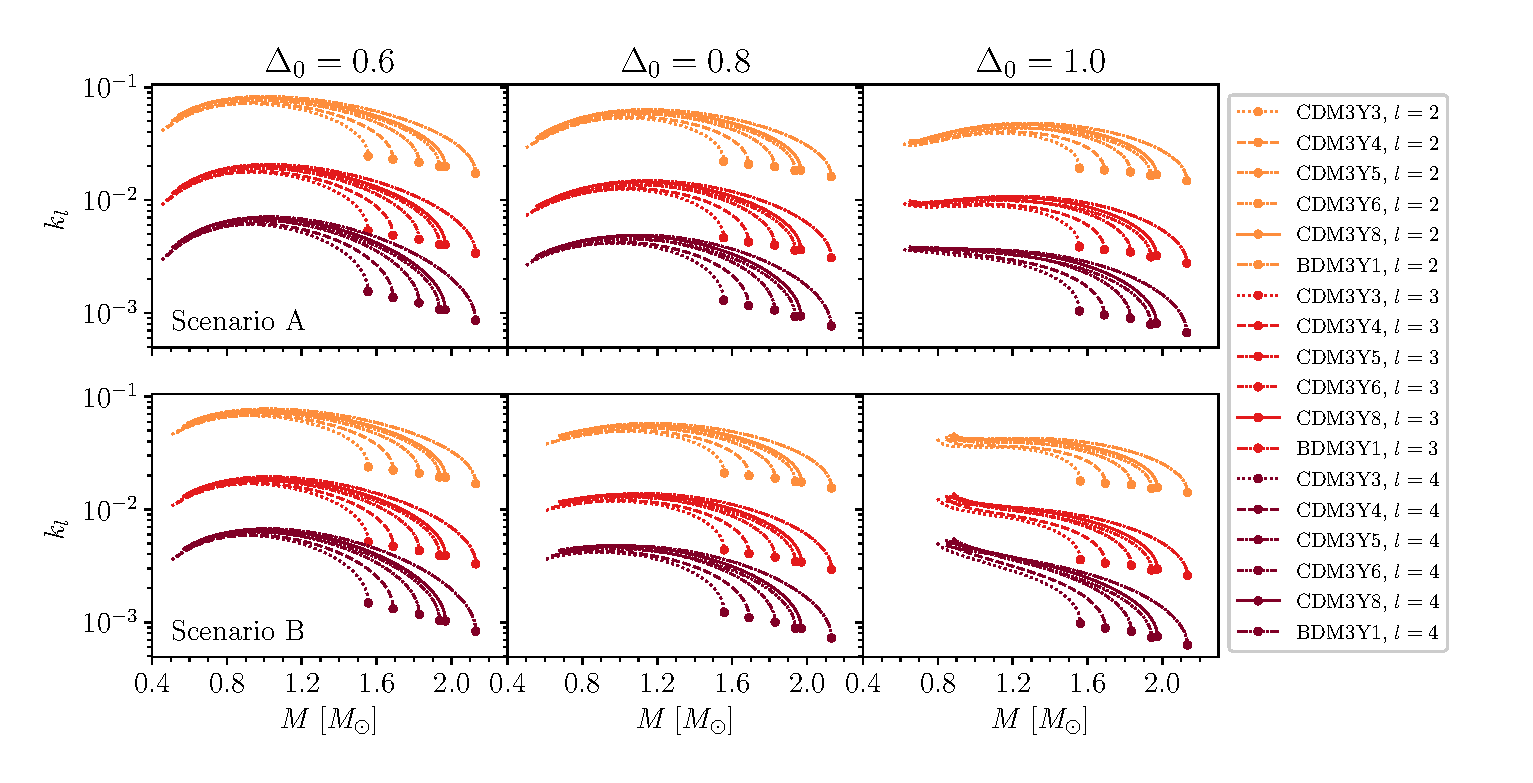
\includegraphics[width=\textwidth]{fig/kl.eps}
        \caption{\gls{GE} tidal Love number at $l$\textsuperscript{th} order $k_l$ as function of magnetar mass computed with 4 density-dependent \gls{NN} interaction versions at different spin polarizations. The dot at the end of each line represents the maximum gravitational mass $M$ of the magnetar generated by the corresponding \gls{EoS}.}
        \label{fig:kl}
\end{figure} 
\begin{figure}[ht!]
    \centering
    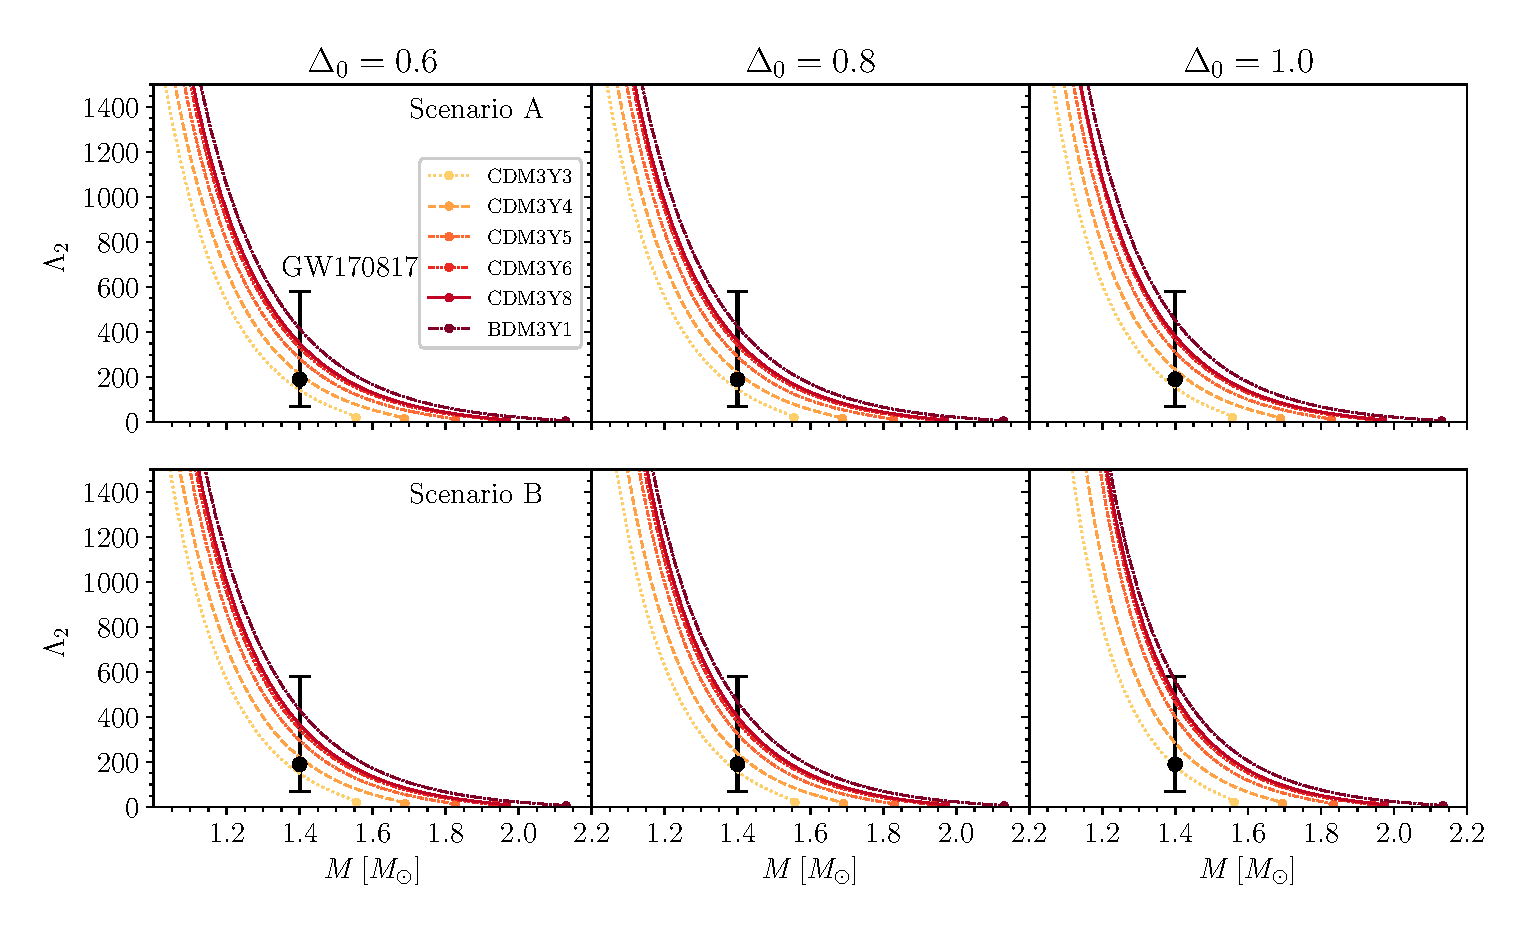
\includegraphics[width=\textwidth]{fig/Lambda2.eps}
    \caption{Dimensionless \gls{GE} tidal deformability parameter of 2\textsuperscript{nd} order $\Lambda_2$ of different CDM3Y$n$ models with varying $\Delta$. The vertical bar is the empirical tidal deformability constraint $\Lambda_2 \approx 190_{-120}^{+390}$ at $1.4M_\odot$, obtained from the Bayesian analysis of GW170817 data with 90\% confidence level \citep{abbott2018gw170817}.}
    \label{fig:Lambda2}
\end{figure} 
The results for \gls{GE} tidal Love number's dependence on \gls{NS}'s gravitational mass arose from 4 versions of the \gls{EoS} are shown in Figure \ref{fig:kl}. Similar to \cite{perot2021role}, in this result, it is clear that the higher the order $l$, the less impactful the Love number $k_l$ is for the tidal properties of the \gls{NS}, i.e. $k_l$ tends to be smaller by an order of magnitude than $k_{l-1}$, as expected from the multipole expansion. The 2\textsuperscript{nd} order is consequently dominant compared to the others. Between two scenarios A and B, at partial polarization of $\Delta_0 = 0.6$, the difference in $k_l$ of the same order is insignificant, except for the small difference in the low mass section. On the other hand, for the case of higher spin polarity in the \gls{NS} surface, the results are much more distinguishable, as the computation with scenario B gives rise to a ``steeper'' curve of $k_l$. Furthermore, in general, the maximum values of $k_l$ are at the common gravitational mass $M$ at all orders computed so far, and this value of $M$ seems to only depends on the value of $\Delta_0$, where the position of maximum $k_l$ tends to be shifted to a higher $M$ as $\Delta_0$ increases. Among these tidal parameters, the only one that has been constrained by far is the dominant 2\textsuperscript{nd} order Love number, which is investigated through the closely related dimensionless tidal deformability parameter of second order $\Lambda_2$ \eqref{eq:Lambda} and whose results are given in Figure \ref{fig:Lambda2}. In the study of \cite{abbott2018gw170817}, the range of $\Lambda_2$ is accepted to be $\Lambda_2 \approx 190^{+390}_{-120}$ at $M=1.4M_\odot$. It is interesting to note that for all cases in this study, this constraint tolerates all \glsplural{EoS} and scenarios, as well as the value of $\Delta_0$, thus no further exclusion can be done with this parameter. It's worth mentioning that the nuclear incompressibility $K$ plays a significant role in determining the tidal deformability $\Lambda_2$ as when $K$ varies from version to version (CDM3Y4 to CDM3Y8), the value of $\Lambda_2$ increases by $\approx 3$ times for the scenario A of $\Delta_0 = 0.6$ case, the same can be said for the different configuration of $\Delta(n_b)$. Testing the values of $k_l$ at higher orders can also be done by evaluating the tidal correction of the \gls{GW} waveform from inspiralling \glsplural{NS} within the PN theory, i.e. the \gls{GE} contribution of order $(2l+1)$PN to the phase of \gls{GW} signal is \citep{perot2021role, yagi2014multipole}
\begin{equation}
    \Psi_l = - \sum^{2}_{i=1} \left[ \frac{5}{16} \frac{(2l-1)!! (4l+3)(l+1)}{(4l-3)(2l-3)} \Lambda_{l,i} X_i^{2l-1} x^{2l - 3/2} + \frac{9}{16} \delta_{l2} \Lambda_{2, i} \frac{X_i^4}{\eta} x^{5/2} \right] + \mathcal{O}(x^{2l-1/2})
\end{equation}
where $i=1,\,2$ is the index distinguishing the two \glsplural{NS} of the system, $x=\left( G\pi Mf/c^3 \right)^{2/3}$, $f$ is the \gls{GW} signal frequency, $M=M_1 + M_2$, $X_i = M_i/M$ and $\eta = M_1 M_2/M^2$.

The gravito-magnetic tidal Love numbers $j_l$ contribute more weakly to the \gls{GW} phase compared to that of their \gls{GE} counterpart, as the \gls{GM} terms only appear from higher orders of $(2l+2)$PN, where the first correction at 6PN is given by \citep{perot2021role,yagi2017erratum}
\begin{equation}
    \tilde{\Psi}_2 = \sum^{2}_{i=1} \frac{5}{224} \sigma_{2,i} \frac{X_i^4}{\eta} \left( X_i - 1037X_j \right)x^{7/2} + \mathcal{O}(x^{9/2})
\end{equation}
\begin{figure}[ht!]
        \centering
        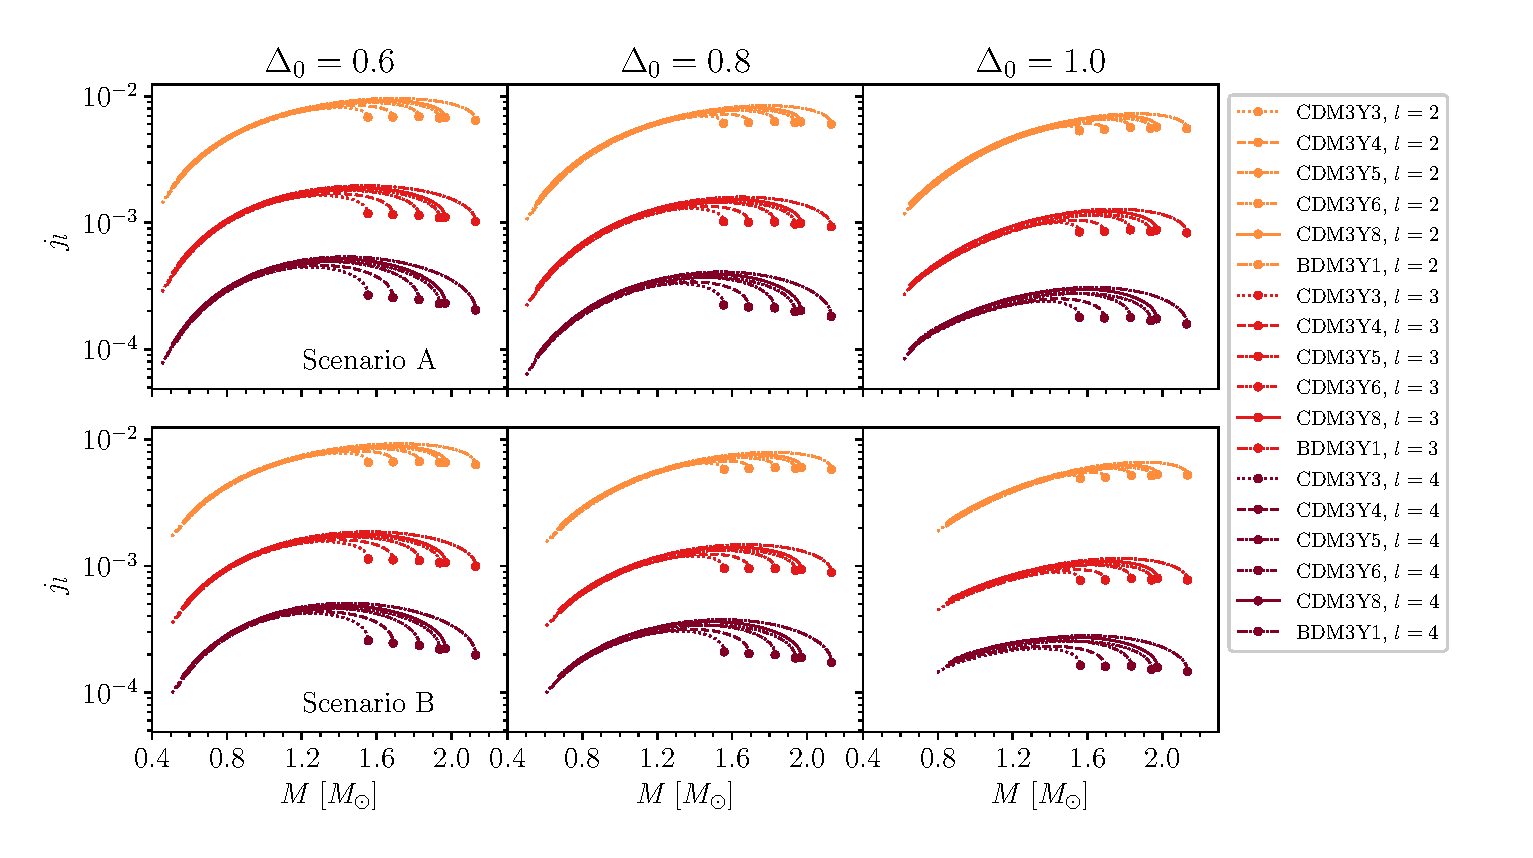
\includegraphics[width=\textwidth]{fig/jl_stat.eps}
        \caption{\gls{GM} tidal Love number at $l$\textsuperscript{nd} order $j_l$ as function of \gls{NS} mass computed with CDM3Y$n$ models of \emph{strictly static fluid} at different polarizations.}
        \label{fig:jl_stat}
\end{figure} 
\begin{figure}[ht!]
        \centering
        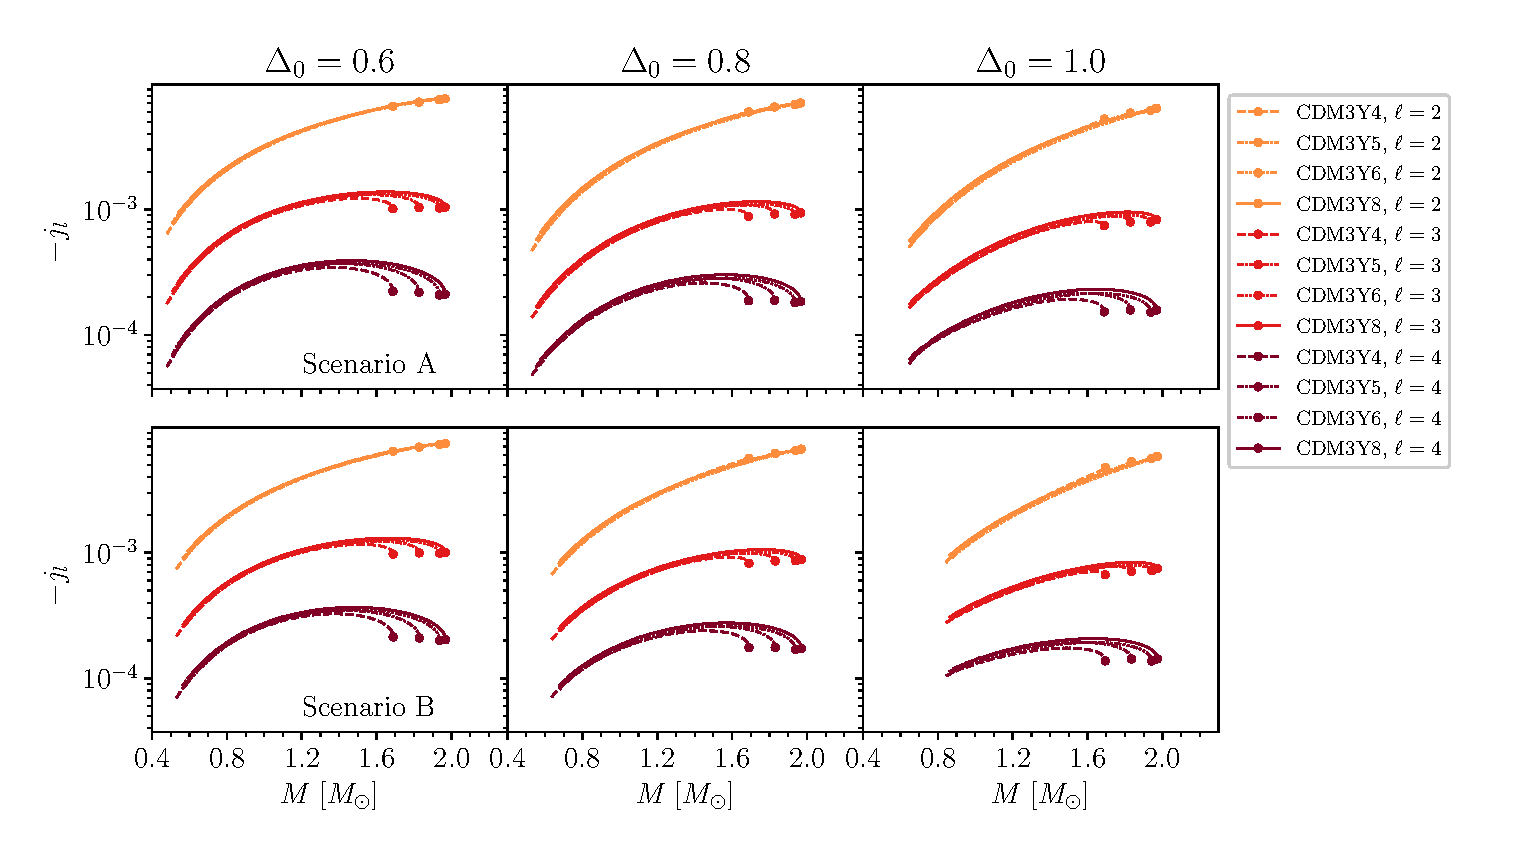
\includegraphics[width=\textwidth]{fig/jl_irrot.eps}
        \caption{\gls{GM} tidal Love number at $l$\textsuperscript{nd} order $j_l$ as function of \gls{NS} mass computed with CDM3Y$n$ models of \emph{irrotational fluid} at different polarizations.}
        \label{fig:jl_irrot}
\end{figure} 
The \gls{GM} tidal Love numbers of second, third and fourth order computed with 4 different \glsplural{EoS} are shown in Figure \ref{fig:jl_stat} for strictly static fluid and \ref{fig:jl_irrot} for irrotational fluid. Apart from the same trends as the \gls{GE} tidal Love numbers discussed previously, the \gls{GM} Love numbers' values do not have much variation as $\Delta_0$ increases in each scenario, as the shape of each curves in Figure \ref{fig:jl_stat} doesn't differ far from each others except for the difference in range of gravitational mass $M$. The value of $j_l$ corresponding to the \gls{GM} pertubation of irrotational fluid (Figure \ref{fig:jl_irrot}), on the other hand, stands out from the other two types of Love numbers, where its value is completely negative, albeit having the same magnitude as that of static fluid, this type of fluid motion is stated to be more realistic in this case due to it being driven by the tides \citep{perot2021role,pani2018magnetic}. In this case, the lines traced by each interation appear to reach maximum value at the maximum $M$ at the leading terms only, rather than having a local maxima in between. The dominance of the 2\textsuperscript{nd} order terms are clear in all cases, where the difference of around one order of magnitude is maintained. Notably, for the \gls{GM} terms corresponding with each \gls{NN} interaction, at higher order $l$, the \gls{NS} mass at maximum $j_l$ seems to become smaller. One more interesting result is that the magnitudes of $j_l$ for two types of fluid are also comparable but is smaller than their \gls{GE} counterpart by one order of magnitude, similar to the conclusion reached by \cite{perot2021role}.


        \chapter{Results and Discussions}
        \label{chap:result}
        Under the condition of \textbeta-stable, the proton's contribution $x_p = \rho_p/\rho_b$ to the baryon density of of \gls{NM} is given by Figure \ref{fig:xp}
\begin{figure}[ht!]
        \centering
        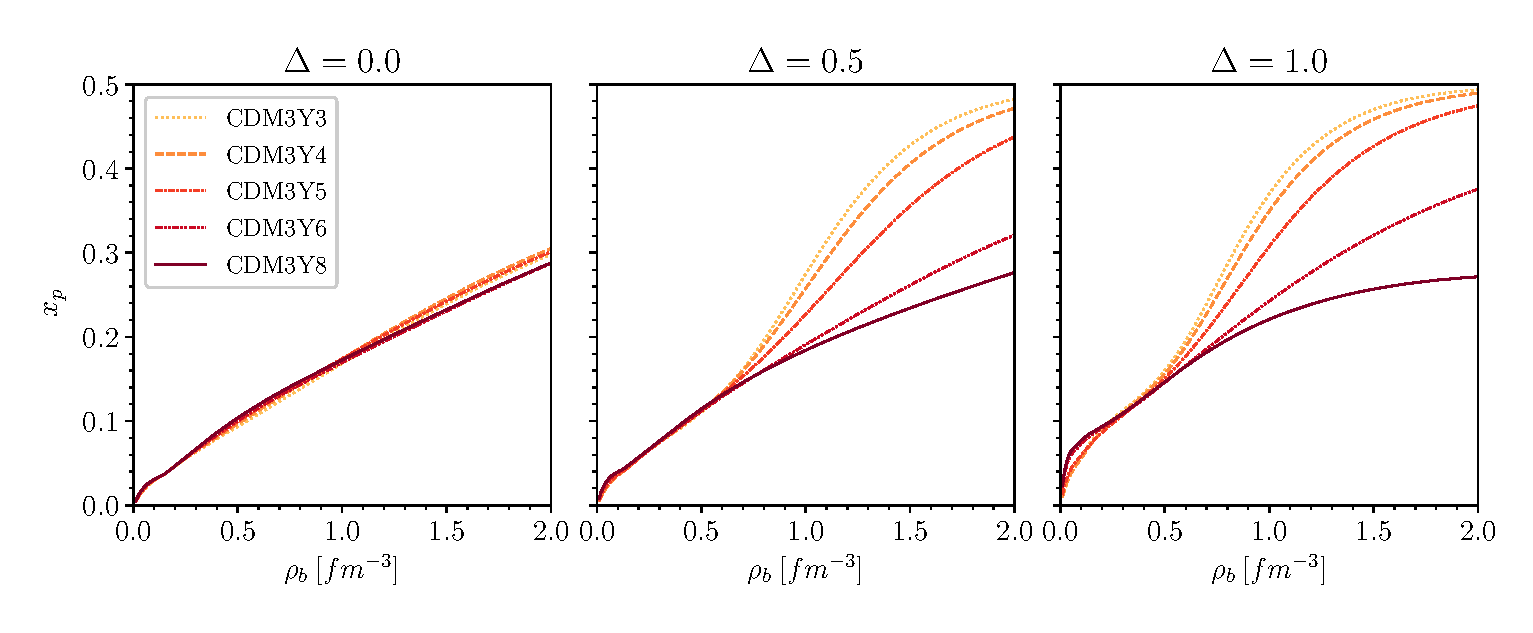
\includegraphics[width=\textwidth]{fig/xp.eps}
        \caption{Proton fraction $x_p$ of \textbeta-stable \gls{NM} at different baryon density and spin polarity for CDM3Y$n$ interactions. The lower horizontal lines are the \gls{DU} threshold. The dot at the end of each line corresponds to the highest mass \gls{NS}'s central density of each model.}
        \label{fig:xp}
\end{figure} 
\begin{figure}[ht!]
        \centering
        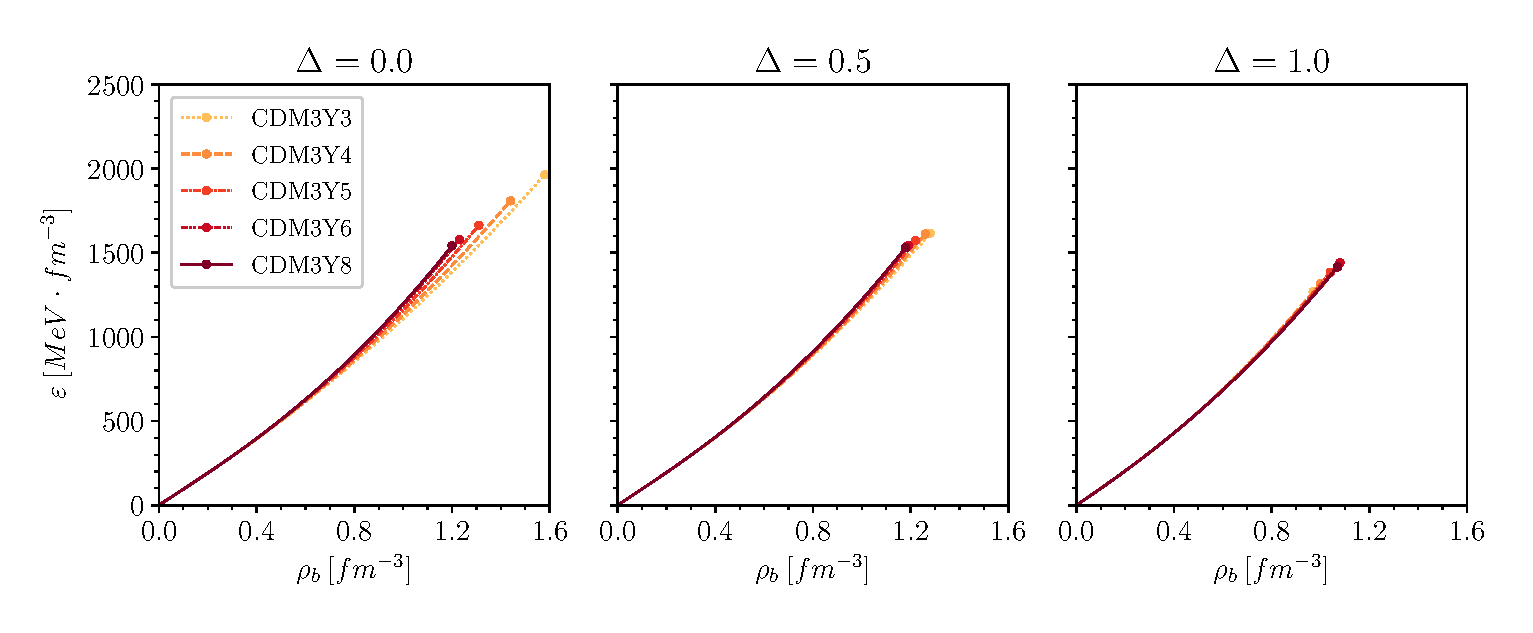
\includegraphics[width=\textwidth]{fig/E.eps}
        \caption{Total mass-energy density $\varepsilon$ of \textbeta-stable \gls{NM} at varying spin polarity with different interaction models. The dot at the end of each line corresponds to the highest mass \gls{NS}'s central density of each model.}
        \label{fig:e}
\end{figure} 
\begin{figure}[ht!]
        \centering
        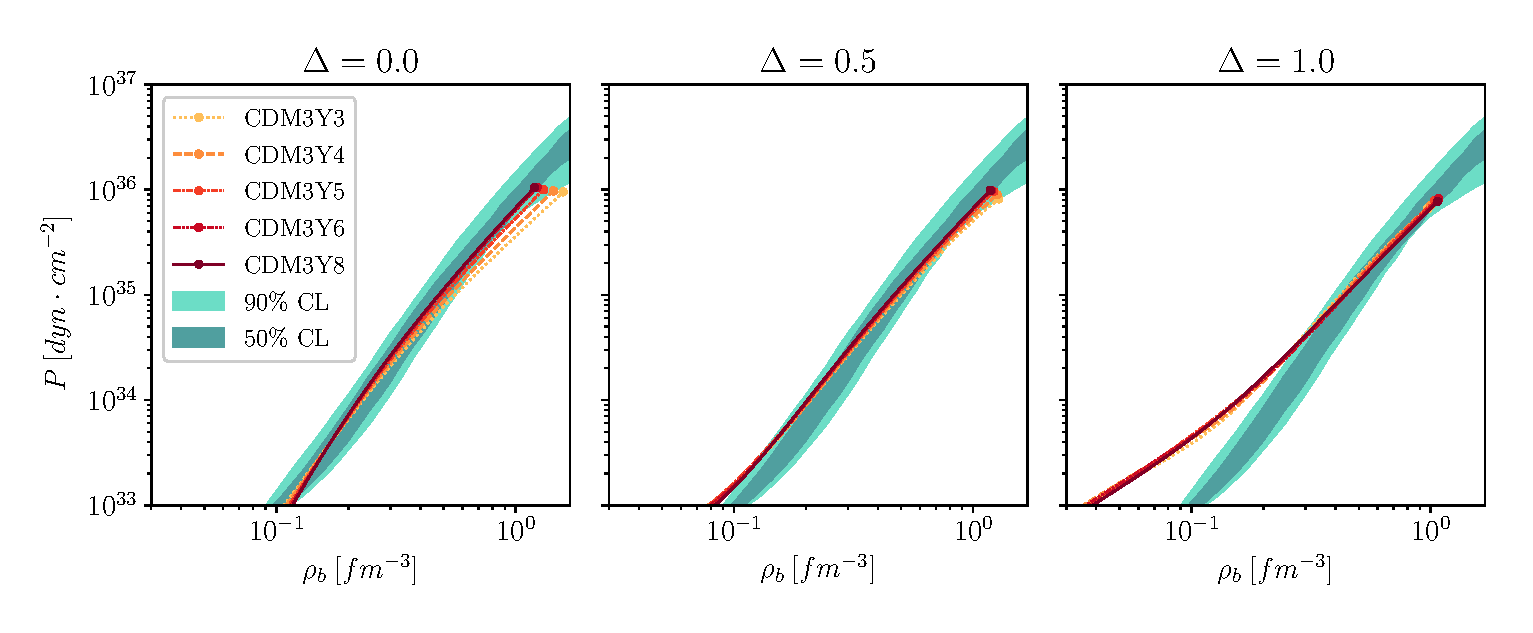
\includegraphics[width=\textwidth]{fig/P.eps}
        \caption{Same as Figure \ref{fig:e} for the pressure $P$.}
        \label{fig:p}
\end{figure} 
\begin{figure}[ht!]
        \centering
        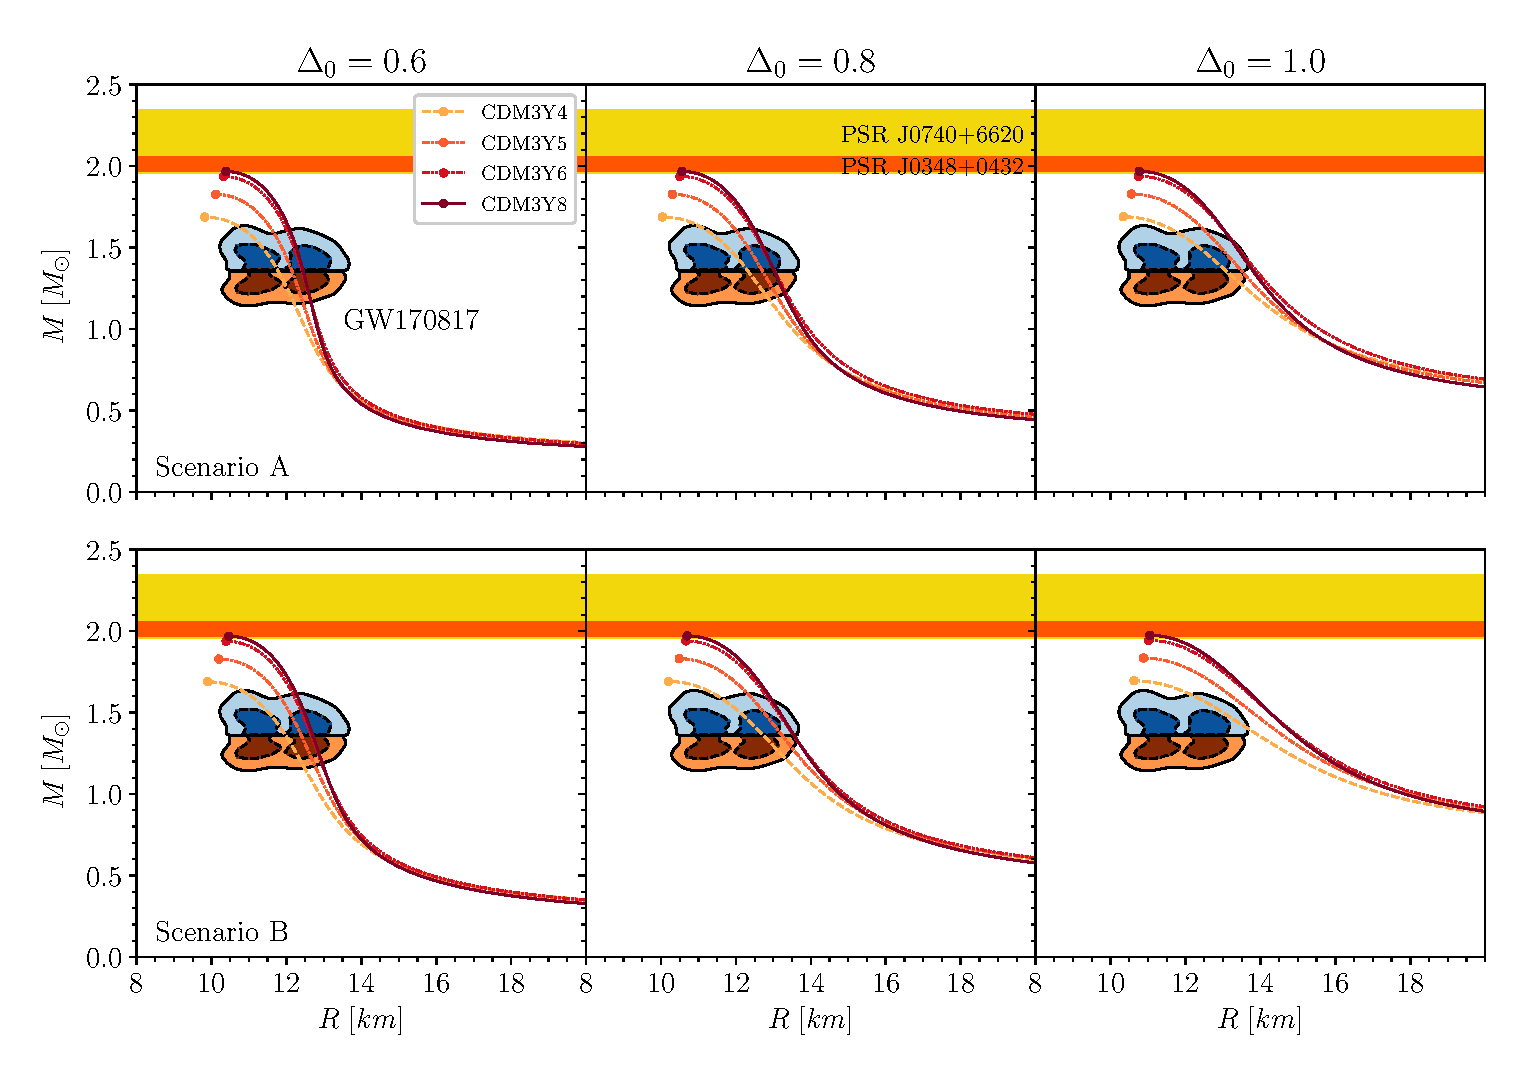
\includegraphics[width=\textwidth]{fig/MR.eps}
        \caption{The relation between gravitational mass $M$ and the radius $R$ of the \gls{NS} according to the corresponding model and polarity.}
        \label{fig:mr}
\end{figure} 
\begin{figure}[ht!]
        \centering
        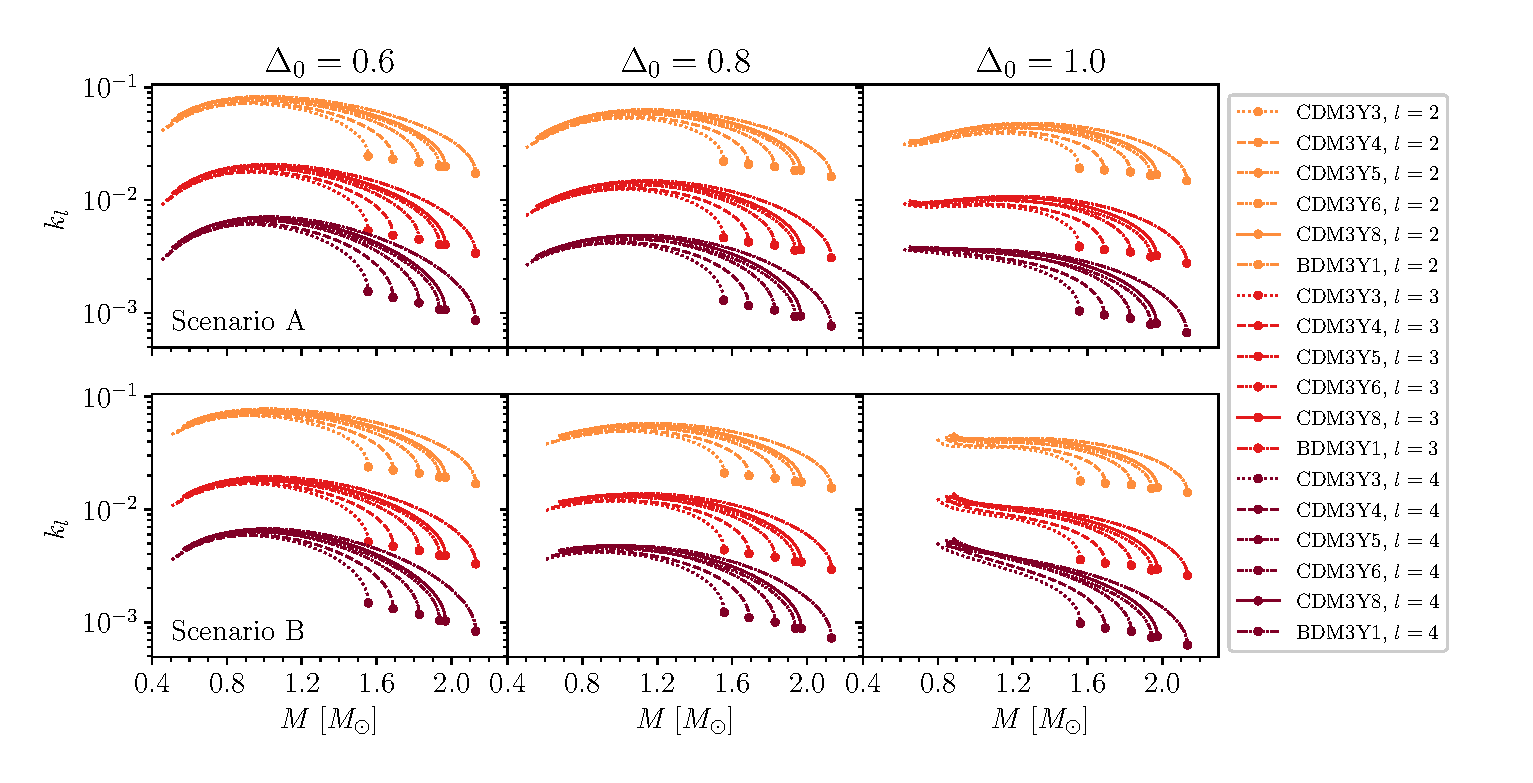
\includegraphics[width=\textwidth]{fig/kl.eps}
        \caption{\gls{GE} tidal Love number at $l$\textsuperscript{th} order $k_l$ as function of \gls{NS} mass computed with CDM3Y$n$ models at different spin polarities.}
        \label{fig:kl}
\end{figure} 
\begin{figure}[ht!]
        \centering
        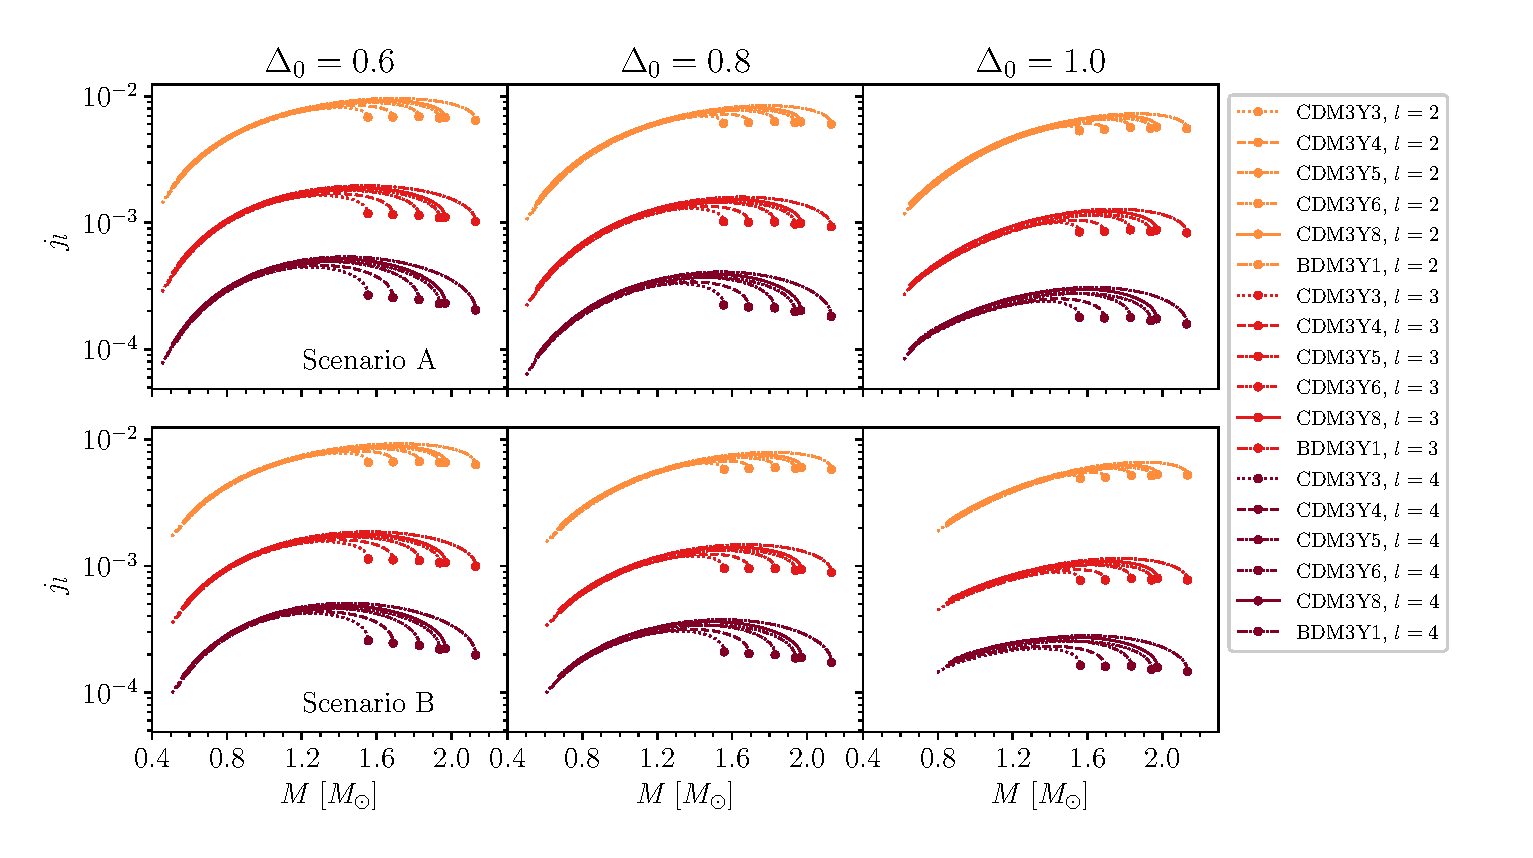
\includegraphics[width=\textwidth]{fig/jl_stat.eps}
        \caption{\gls{GM} tidal Love number at $l$\textsuperscript{nd} order $j_l$ as function of \gls{NS} mass computed with CDM3Y$n$ models of \emph{strictly static fluid} at different polarities.}
        \label{fig:jl_stat}
\end{figure} 
\begin{figure}[ht!]
        \centering
        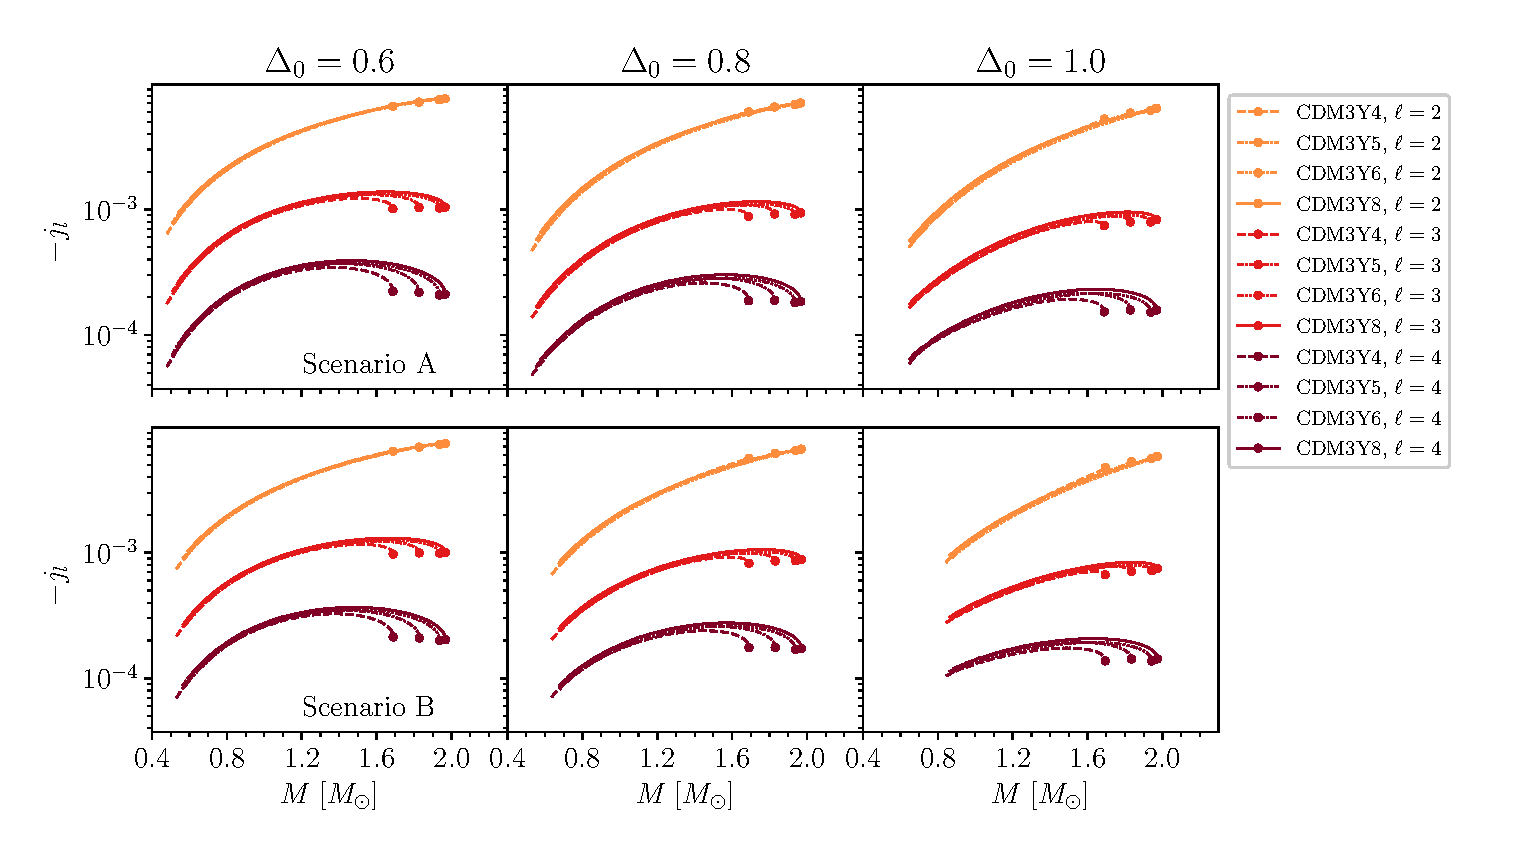
\includegraphics[width=\textwidth]{fig/jl_irrot.eps}
        \caption{\gls{GM} tidal Love number at $l$\textsuperscript{nd} order $j_l$ as function of \gls{NS} mass computed with CDM3Y$n$ models of \emph{irrotational fluid} at different polarities.}
        \label{fig:jl_irrot}
\end{figure} 

        
        \chapter{Conclusions}
        \label{chap:conclusion}
        By extending the 4 current versions of density-dependent \gls{NN} interaction \citep{tan2021equation}, we have been able to include the description of spin polarization effect of \gls{NS} matter under strong magnetic field over a wider range of $K$ into the \gls{EoS} of \gls{NM} using the nonrelativistic \gls{HF} formalism. In general, concerning the \gls{EoS} of \gls{NM}, the empirical ranges deduced for symmetry energy $S$, energy per baryon of symmetric \gls{NM} $E/A$ and total pressure $P$ seem to favor partial to zero polarization, or in particular, the cases with lower $\Delta$ overall. Among these 4 versions of \gls{EoS}, the CDM3Y4 interaction is very unlikely to occur in reality, as the \gls{EoS} generated by these interactions are usually outside of the 90\% \gls{CFL} boundary obtained from astrophysical observation and analysis at high density.

The density-dependence of the polarization $\Delta$ is also taken into account by using different situations regarding the localization of magnetic field at the surface of magnetar \citep{tan2020spin}, which eventually eliminates the possibility of total polarization at the magnetar's surface, i.e. $\Delta_0\approx 1.0$. The macroscopic properties of the \gls{NS}, on the other hand, only the cases of partial polarization at the scenario A succeed in staying within the GW170817 constraint \citep{abbott2018gw170817}, which supports the suggestion of the blue kilonova ejecta of GW170817 coming from a magnetar \citep{metzger2018magnetar,tan2020spin}. Furthermore, only the CDM3Y6 and CDM3Y8 in these scenarios can come close to satisfy the lower mass limit of the two heaviest pulsars ever observed, i.e. \gls{PSR} J0348+0432 and \gls{PSR} J0740+6620. The tidal deformability parameter $\Lambda_2$, surprisingly, do not provide further constraint, as all cases are within the accepted range obtained by \cite{abbott2018gw170817}. Beside, higher orders of multipoles up to the 4\textsuperscript{th} order have been investigated for both gravito-electric and gravito-magnetic tidal perturbations. The common diminishing effects as the order $\ell$ increases are founded for all cases, as well as the dominance of the \gls{GE} tidal Love numbers in magnitude compared to the \gls{GM} ones, which is in agreement with the contribution of each term in the phase of \gls{GW} signal \citep{abdelsalhin2018post} as only the $\ell=2$ order of GE tidal deformation contributes significantly enough to be detectable by current measurements. The observation of \gls{GM} tidal deformability can be possibly used as an additional test for Einstein's theory of \gls{GR}, since these effects are not presented in Newtonian physics. More information on the \gls{EoS} of \gls{NS} matter can also be further constrained with the potential observation of the higher order terms, which might be possible with the 3\textsuperscript{rd}-generation \gls{GW} detectors \citep{maggiore2020science}.

In conclusion, regarding the research progress made within this Thesis, all of the objectives demanded have been fulfilled. Additionally, there are several ways in which this topic can be further expanded in the future, i.e.
\begin{itemize}
    \item Accurately calculation of the density dependence of $\Delta(n_b)$,
    \item Extending to a model of hot \textbeta-stable \gls{NS} matter ($T>0\:K$),
    \item Describing the quark-matter core in the interior core of \gls{NS}.
\end{itemize}


        \clearpage
        \bibliographystyle{apalike}
        \bibliography{ref}
\end{document}
